% ============================================================
%  PFE Report -- Object-Aware Latent Adversarial Attack on YOLOv8
%  Author : Mohamed Aziz Brahmi
%  Compile: pdflatex -> bibtex -> pdflatex x2  (or use Overleaf)
% ============================================================

\documentclass[12pt,a4paper]{report}

% -- Encoding & fonts -----------------------------------------
\usepackage[utf8]{inputenc}
\usepackage[T1]{fontenc}
\usepackage{lmodern}
\usepackage{microtype}

% -- Page layout ----------------------------------------------
\usepackage[
  a4paper,
  top=2.5cm, bottom=2.5cm,
  left=3cm,  right=2.5cm,   % wider left margin for binding
  headheight=15pt
]{geometry}

% -- Line spacing ---------------------------------------------
\usepackage{setspace}
\onehalfspacing

% -- Mathematics ----------------------------------------------
\usepackage{amsmath,amssymb,bm}

% -- Graphics -------------------------------------------------
\usepackage{graphicx}
\usepackage[table]{xcolor}

% -- Tables ---------------------------------------------------
\usepackage{booktabs}
\usepackage{array}
\usepackage{multirow}

% -- Code listings --------------------------------------------
\usepackage{listings}
\lstset{
  basicstyle=\ttfamily\small,
  breaklines=true,
  frame=single,
  numbers=left,
  numberstyle=\tiny,
  keywordstyle=\bfseries\color{blue!70!black},
  commentstyle=\itshape\color{gray},
  stringstyle=\color{orange!80!black}
}

% -- Headers & footers ----------------------------------------
\usepackage{fancyhdr}
\pagestyle{fancy}
\fancyhf{}
\fancyhead[L]{\small\nouppercase{\leftmark}}
\fancyhead[R]{\small Final-Year Project -- M.A. Brahmi}
\fancyfoot[C]{\small\thepage}
\renewcommand{\headrulewidth}{0.4pt}

% -- Chapter title formatting ---------------------------------
\usepackage{titlesec}
\titleformat{\chapter}[display]
  {\normalfont\huge\bfseries}
  {\chaptertitlename\ \thechapter}{18pt}{\Huge}
\titlespacing{\chapter}{0pt}{30pt}{20pt}

% -- Hyperlinks (must be near last) ---------------------------
\usepackage[
  colorlinks=true,
  linkcolor=blue!60!black,
  citecolor=green!40!black,
  urlcolor=blue!60!black
]{hyperref}

% -- Bibliography (natbib, numeric style) ---------------------
\usepackage[numbers,sort&compress]{natbib}

% -- Utility --------------------------------------------------
\usepackage{enumitem}
\usepackage{caption}
\captionsetup{font=small, labelfont=bf}

% -- Figure path ----------------------------------------------
\graphicspath{{figures/}}

% -- Custom commands ------------------------------------------
\newcommand{\Ldet}{\mathcal{L}_{\text{det}}}
\newcommand{\Lperc}{\mathcal{L}_{\text{perc}}}
\newcommand{\Lreg}{\mathcal{L}_{\text{reg}}}
\newcommand{\Mz}{M_z}
\newcommand{\xadv}{x'}
\newcommand{\zadv}{z_{\text{adv}}}

% -- Draft watermark (comment out for final version) ----------
% \usepackage{draftwatermark}
% \SetWatermarkText{DRAFT}\SetWatermarkScale{3}\SetWatermarkColor[gray]{0.92}

% ============================================================
\begin{document}

% -- Plain style for front matter -----------------------------
\pagestyle{plain}

% ============================================================
%  TITLE PAGE
% ============================================================
\begin{titlepage}
  \centering
  \vspace*{1cm}

  % University logo -- replace path with your actual logo file
  % \includegraphics[width=4cm]{logo_university.png}\\[1cm]

  {\large \textsc{Université de Tunis El Manar}}\\[0.3cm]
  {\large \textsc{Faculté des Sciences de Tunis (FST)}}\\[0.5cm]
  \rule{\linewidth}{0.4pt}\\[0.4cm]

  {\huge \bfseries Object-Aware Latent Adversarial Attack\\[0.3cm]
  on YOLOv8}\\[0.4cm]

  \rule{\linewidth}{0.4pt}\\[1cm]

  {\large \textit{Final-Year Engineering Internship Report (PFE)}}\\[0.3cm]
  {\large \textit{Domain: Computer Vision -- Adversarial Machine Learning}}\\[1.5cm]

  \begin{tabular}{rl}
    \textbf{Author:}      & Mohamed Aziz Brahmi \\[4pt]
    \textbf{Supervisor:}  & Mme.~Leila Ben Othman \\[4pt]
    \textbf{Institution:} & University of Prince Mugrin \\[4pt]
    \textbf{Academic year:} & 2025 -- 2026 \\
  \end{tabular}

  \vfill
  {\large 8 June 2026}
\end{titlepage}

% ============================================================
%  FRONT MATTER
% ============================================================
\setcounter{page}{1}
\pagenumbering{roman}

% -- Abstract -------------------------------------------------
\chapter*{Abstract}
\addcontentsline{toc}{chapter}{Abstract}

We propose a minimal, reproducible adversarial attack that perturbs only the bounding-box
latents of a frozen Stable-Diffusion VAE under a vanishing-confidence objective, causing all
originally detected objects to disappear from a YOLOv8 detector's output while keeping
perturbations imperceptible inside the masked region. Experiments on UA-DETRAC, a
large-scale vehicle-surveillance benchmark, show that our method matches or exceeds
pixel-space PGD on Detection Failure Rate while reducing perceptual distortion inside the
attacked region as measured by masked LPIPS (0.165 for the best latent configuration vs.\ $\geq$0.095 for PGD at matched perturbation budget).

\vspace{1em}
\noindent\textbf{Keywords:} adversarial examples, object detection, YOLOv8, latent diffusion,
VAE, UA-DETRAC, false-negative attack, perturbation stealth.

% -- Acknowledgements -----------------------------------------
\chapter*{Acknowledgements}
\addcontentsline{toc}{chapter}{Acknowledgements}

I would like to express my sincere gratitude to my supervisor, Mme.~Leila Ben Othman, for her guidance, constructive feedback, and constant availability throughout this project. I am grateful to the University of Prince Mugrin for providing the computational infrastructure that made the deep-learning experiments presented in this report possible. I also thank the open-source communities behind Ultralytics YOLOv8, Stable Diffusion, and PyTorch, whose tools formed the technical foundation of this work. Finally, I thank my family for their unwavering support and encouragement.

% -- Table of contents ----------------------------------------
\tableofcontents
\listoffigures      % remove if no figures yet
\listoftables       % remove if no tables yet

% -- Switch to arabic page numbering --------------------------
\clearpage
\pagenumbering{arabic}
\setcounter{page}{1}
\pagestyle{fancy}

% ============================================================
%  CHAPTER 1 -- RESUME
% ============================================================
% ============================================================
%  CHAPTER 1 — General Context and Internship Presentation
% ============================================================
% ============================================================
%  INTRODUCTION GÉNÉRALE (unnumbered)
% ============================================================
\chapter*{General Introduction}
\addcontentsline{toc}{chapter}{General Introduction}
\label{ch:intro_gen}

The deployment of deep learning systems in safety-critical infrastructures
has created a pressing need to understand their adversarial vulnerabilities.
Object detection models --- and in particular the YOLO family of single-stage
detectors \cite{redmon2016you,jocher2023ultralytics} --- now underpin
autonomous vehicle perception, intelligent traffic surveillance, and
public-space monitoring. Since the seminal work of Goodfellow et al.\
\cite{goodfellow2014explaining}, it has been established that these models
can be deceived by \emph{adversarial perturbations}: small, structured
modifications to input images that induce incorrect predictions while
remaining imperceptible to a human observer. Madry et al.\
\cite{madry2018towards} formalised this threat as a min-max optimisation
problem, giving rise to the Projected Gradient Descent (PGD) attack that
remains the de facto white-box baseline to this day.

Among the failure modes an adversary can induce in an object detector, the
\emph{false-negative regime} --- causing the model to silently miss every
object that is genuinely present --- carries exceptional safety implications.
A surveillance camera that reports no vehicles provides no anomaly signal
to downstream monitoring systems; a missed pedestrian detection in autonomous
driving can be life-threatening \cite{placeholder_adas}. Yet existing
adversarial attacks on detectors focus predominantly on false positives or
localisation errors \cite{xie2017adversarial,li2020robust}, and classical
pixel-space attacks such as PGD introduce structured high-frequency noise
detectable by learned perceptual metrics \cite{zhang2018unreasonable}, even
at tight $\ell_\infty$ budgets. This work addresses both challenges
simultaneously by operating in the latent space of the Variational
Autoencoder (VAE) component of Stable Diffusion \cite{rombach2022high},
which acts as a fixed manifold prior that biases perturbations toward
perceptually natural directions.

Three concrete contributions are presented:

\medskip
\noindent\textbf{N1 --- Object-aware latent perturbation.}
The perturbation is restricted to the latent sub-tensor corresponding to
detected bounding boxes via stride-8 max-pool projection, and a paste-back
operator restores background pixels exactly in pixel space. This is the first
method to couple spatial bounding-box constraints with latent-space
optimisation for false-negative suppression in object detection.

\medskip
\noindent\textbf{N2 --- Vanishing-only detection objective.}
A class-level maximum-confidence loss with saturation floor drives every
originally detected class below the NMS confidence threshold without
requiring post-NMS decoding. The objective is minimal, numerically stable,
and directly aligned with the false-negative failure mode.

\medskip
\noindent\textbf{N3 --- Manifold-constrained stealth without diffusion.}
Optimising in the frozen VAE latent space alone --- without text conditioning
or denoising steps --- suffices to produce perturbations biased toward the
natural-image manifold. The best configuration achieves
DFR$_\text{prop} = 9.1\%\pm2.5\%$ on UA-DETRAC \cite{wen2020ua}, outperforming
pixel-space PGD (DFR $\leq1.0\%$) while avoiding the spurious-detection
failure mode entirely.

\medskip
\noindent\textbf{Report organisation.}
Chapter~\ref{ch:context} (\textit{Context and Positioning}) presents the
academic and institutional context, the project objectives, and a gap analysis
that positions the approach relative to existing attacks.
Chapter~\ref{ch:background} (\textit{State of the Art}) reviews the technical
literature and closes with a comparative positioning table.
Chapter~\ref{ch:method} (\textit{Methodology and Implementation}) gives the
full mathematical derivation and a concise description of the modular codebase.
Chapter~\ref{ch:results} (\textit{Experimentation and Results}) reports
experimental results, ablation studies, failure-mode analysis, and threat-model
limitations. The report closes with a Conclusion and research perspectives.

% ============================================================
%  CHAPTER 1 — CONTEXTE ET POSITIONNEMENT
% ============================================================
\chapter{Context and Positioning}
\label{ch:context}
\label{ch:intro}

This chapter presents the academic and institutional context of the internship, defines the three operational objectives that guided the work, describes the deliberate scope refinement toward a focused experimental design, and closes with a gap analysis (Table~\ref{tab:gap_analysis}) that positions this work relative to existing adversarial attack families.

% ------------------------------------------------------------
\section{Academic Framework: The Final-Year Engineering Internship}
\label{sec:pfe-framework}
% ------------------------------------------------------------

The \textit{Projet de Fin d'Études} (PFE) is the capstone requirement of the
engineering curriculum at the Faculté des Sciences de Tunis (FST), Université de Tunis El Manar. It is
designed to bridge the gap between academic training and professional research
practice by embedding students in a real-world technical environment for a
period of approximately six months. During this period, the student is expected
to identify a well-defined engineering or research problem, propose a
technically sound solution, implement it, and evaluate it against meaningful
baselines.

The present internship was carried out in the domain of \textbf{computer vision
and adversarial machine learning} --- two fields that have seen rapid and
simultaneous growth over the past decade. Computer vision provides the
perceptual backbone of a growing number of safety-critical systems, while
adversarial machine learning studies the fragility of these systems to
imperceptible but carefully crafted perturbations. The convergence of these two
fields defines both the scientific motivation and the practical stakes of this
project.

% ------------------------------------------------------------
\section{Host Organization}
\label{sec:host}
% ------------------------------------------------------------

The internship was conducted at the University of Prince Mugrin, Kingdom of Saudi Arabia, under the
supervision of Mme.~Leila Ben Othman. The host environment provided access to the computational resources
and research infrastructure required to carry out deep-learning experiments at
scale, in particular GPU-accelerated training on the UA-DETRAC vehicle
surveillance dataset and inference with large pretrained generative models.

% ------------------------------------------------------------
\section{Project Objectives and Initial Scope}
\label{sec:objectives}
% ------------------------------------------------------------

At the outset of the internship, the project was framed around a central
question in adversarial robustness for object detection:

\begin{quote}
\textit{Is it possible to construct an adversarial perturbation that suppresses
all objects detected by a state-of-the-art detector, while remaining
imperceptible to a human observer --- and can latent-space optimisation improve
the stealth of such an attack compared to classical pixel-space methods?}
\end{quote}

This question is motivated by a concrete safety concern. Modern surveillance
and autonomous driving systems rely on object detectors to make real-time
decisions. An adversary who can cause a detector to \emph{miss} all vehicles or
pedestrians in a scene --- without visibly altering the image --- poses a
serious threat that existing defences are not designed to address. The
false-negative regime, in which detections silently disappear rather than
becoming noisy, is particularly dangerous because it is less likely to trigger
downstream anomaly-detection mechanisms.

Three operational objectives were defined at the start of the internship:

\begin{enumerate}[label=\textbf{O\arabic*.}, leftmargin=*, itemsep=4pt]

  \item \textbf{Domain-specific detector.} Fine-tune a YOLOv8 detector on a
  vehicle-surveillance dataset (UA-DETRAC) to obtain a realistic deployment
  target, rather than attacking generic COCO-pretrained weights. This ensures
  that the experimental setting reflects a plausible real-world scenario.

  \item \textbf{Latent-space attack.} Design an adversarial attack that
  operates in the latent space of a pretrained generative VAE (Stable Diffusion
  VAE), restricted to the spatial footprint of detected objects, and evaluate
  whether this constraint produces perturbations that are both effective and
  perceptually natural.

  \item \textbf{Rigorous comparative evaluation.} Benchmark the proposed method
  against pixel-space baselines (FGSM and PGD, in both full-image and
  mask-restricted variants) under strictly matched perturbation budgets, using
  a set of metrics that cover attack effectiveness, stealth, and
  detection-level impact.

\end{enumerate}

% ------------------------------------------------------------
\section{Scope Evolution and Methodological Focus}
\label{sec:scope-evolution}
% ------------------------------------------------------------

The original project plan spanned three to four months and included a broader
exploration of multiple detector architectures, physical-world patch generation,
and transfer experiments across datasets. As the internship progressed, a
deliberate decision was made to narrow the scope to a single, depth-first
experiment: \textbf{one detector architecture} (YOLOv8n), \textbf{one dataset}
(UA-DETRAC), \textbf{one threat model} (white-box, digital-only), and \textbf{one
generative prior} (the Stable Diffusion VAE encoder--decoder pair).

This refocusing was motivated by the observation, well established in the
adversarial machine learning literature, that methodological rigour and
reproducibility are more scientifically valuable than breadth. A controlled,
fully documented experiment on a single setting allows unambiguous attribution
of observed effects to specific design choices --- a prerequisite for the
ablation studies that constitute a core part of this project's evaluation
protocol.

The practical consequence of this refocusing was a compression of the
experimental timeline: detector training, attack implementation, baseline
comparison, and ablation studies were planned and executed within a
concentrated period, with all code organised into a reproducible repository
(\texttt{minimal\_research/}) built around a single configuration file
(\texttt{configs/default.yaml}).

% ------------------------------------------------------------
\section{Research Positioning: Gap Analysis}
\label{sec:gap_analysis}
% ------------------------------------------------------------

Table~\ref{tab:gap_analysis} summarises the key limitations of existing
adversarial attack families that motivate the three contributions of this work.

\begin{table}[htbp]
  \centering
  \caption{Gap analysis: limitations of existing approaches and how this work addresses each.}
  \label{tab:gap_analysis}
  \small
  \begin{tabular}{@{}p{3.0cm}p{4.8cm}p{4.8cm}@{}}
    \toprule
    \textbf{Existing approach} & \textbf{Key limitation}
      & \textbf{How this work addresses it} \\
    \midrule
    Pixel-space PGD
      & Signed-gradient noise creates spurious detections (negative DFR) at moderate budgets.
      & Frozen VAE decoder acts as implicit low-pass filter; latent perturbations cannot generate structured HF noise. \\
    \addlinespace
    DAG / RAP
      & Perturb all pixels globally; background regions unnecessarily altered.
      & Bounding-box mask + paste-back confine perturbation strictly to detected object footprints. \\
    \addlinespace
    Latent attacks (LSDM)
      & Designed for classifiers; not adapted to structured detector output.
      & Vanishing-only loss targets YOLOv8 pre-NMS logit tensor; no post-NMS decoding required. \\
    \addlinespace
    Full diffusion attacks
      & Require hundreds of NFEs per image (denoising chain + U-Net).
      & Only frozen VAE encoder--decoder used; no text conditioning or denoising. \\
    \addlinespace
    Physical patch attacks
      & Require printed material; incompatible with digital-imperceptibility.
      & Latent manifold prior biases perturbations toward perceptually smooth modifications. \\
    \bottomrule
  \end{tabular}
\end{table}


% ------------------------------------------------------------
\section*{Chapter Summary}
\addcontentsline{toc}{section}{Chapter Summary}
% ------------------------------------------------------------

This chapter has established the full institutional and scientific context of
the internship.  The project originates from a concrete surveillance
security problem — the fragility of YOLOv8-based vehicle detection to
imperceptible digital perturbations — and was carried out during a six-month
placement within an academic research environment. The three operational
objectives (effectiveness, imperceptibility, and rigorous evaluation) guided
every design decision made in subsequent chapters. The scope was deliberately
narrowed from a broad adversarial ML survey to a focused latent-space attack
against false-negative suppression, a gap clearly identified in the
comparative Table~\ref{tab:gap_analysis}. Chapter~\ref{ch:background}
surveys the theoretical and algorithmic background that underpins this
choice.

% ============================================================
%  CHAPTER 2 — ÉTAT DE L'ART
% ============================================================
\chapter{State of the Art}
\label{ch:background}

This chapter surveys the technical foundations on which the proposed attack is built, covering the YOLO detector family, adversarial perturbation theory, detector-specific attack methods, latent-space and generative adversarial approaches, and the role of the Stable Diffusion VAE as a manifold prior. The chapter closes with a comparative positioning table (Section~\ref{sec:positioning}).

% ------------------------------------------------------------
\section{Object Detection with YOLO Architectures}
\label{sec:yolo}
% ------------------------------------------------------------

\subsection{From R-CNN to Single-Stage Detectors}

Modern object detection frameworks can be broadly divided into two families:
two-stage (region-proposal) architectures, pioneered by R-CNN
\cite{girshick2014} and its successors Fast R-CNN and Faster R-CNN, and
single-stage architectures that predict bounding boxes and class labels in a
single forward pass over the image. Two-stage pipelines achieve high accuracy
by first proposing candidate regions and then refining each proposal
independently; however, this separation introduces computational overhead that
limits throughput in real-time applications. Single-stage detectors, by
collapsing region proposal and classification into one network, achieve
substantially higher frame rates with only modest accuracy penalties.

The YOLO (You Only Look Once) paradigm, introduced by Redmon et al.\
\cite{redmon2016}, established the template for the single-stage approach.
The original YOLOv1 divided the input image into a fixed $S \times S$ grid,
with each cell predicting $B$ bounding boxes and $C$ class-conditional
probabilities simultaneously. Although the spatial granularity of YOLOv1 was
limited, its end-to-end design enabled real-time inference at 45 frames per
second on contemporary GPU hardware -- a threshold unattainable for two-stage
competitors. Subsequent versions (YOLOv2 through YOLOv5) progressively
introduced anchor-box priors, multi-scale feature fusion, batch normalisation,
and backbone improvements, each iteration widening the accuracy--speed
Pareto frontier.

\subsection{YOLOv8: Architecture and Design Principles}
\label{subsec:yolov8}

YOLOv8, released by Ultralytics in 2023 \cite{jocher2023}, represents the
most recent iteration of the family and is the detector targeted in this
work. Its design diverges from YOLOv5 in three significant respects.

\textbf{Anchor-free detection head.} Unlike its predecessors, YOLOv8 adopts
an anchor-free prediction paradigm \cite{tian2019fcos}, predicting box
coordinates as direct offsets from the centre of each grid cell rather than
relative to pre-defined anchor templates. This eliminates the need for anchor
hyper-parameter tuning and reduces the number of redundant predictions that
must be suppressed by non-maximum suppression (NMS).

\textbf{Decoupled head.} YOLOv8 separates the classification and box
regression branches into two parallel convolutional heads, a design choice
empirically shown to improve convergence and final accuracy by reducing the
conflicting gradient signals that arise when a single head must solve both
sub-tasks simultaneously.

\textbf{C2f backbone module.} The backbone replaces the earlier CSP (Cross
Stage Partial) bottleneck with a C2f (Cross Stage Feature Fusion) module that
introduces additional gradient flow paths, improving feature reuse without
proportionally increasing parameter count.

For the adversary, the anchor-free multi-scale prediction structure of YOLOv8
is particularly important. The model produces outputs at three spatial scales
(stride-8, stride-16, stride-32), each yielding a tensor of shape
$\tfrac{H}{s} \times \tfrac{W}{s} \times (4 + C)$ per scale, where $C$ is
the number of object classes and the four channels encode centre-offset and
log-scale box dimensions. Confidence scores for the presence of any object
(objectness) are \emph{not} predicted as a separate channel in YOLOv8; class
probabilities implicitly incorporate detection confidence. This architectural
detail is consequential for adversarial loss design, as discussed in
Chapter~\ref{ch:method}.

\subsection{Non-Maximum Suppression and Post-Processing}

The raw output of YOLOv8 at inference time contains many overlapping
candidate detections. Non-maximum suppression (NMS) resolves this redundancy
by iteratively retaining the highest-scoring box and suppressing all
candidates whose intersection-over-union (IoU) with the retained box exceeds a
threshold $\tau_{\text{NMS}}$. From the adversarial perspective, NMS acts as
a non-differentiable bottleneck: gradients cannot be back-propagated through
the discrete box-selection logic. This motivates attacking the raw logit
tensor prior to NMS, as done in this work, rather than constructing a loss
over post-NMS detections.

% ------------------------------------------------------------
\section{Adversarial Machine Learning: Foundations}
\label{sec:adv_foundations}
% ------------------------------------------------------------

\begin{figure}[htbp]
  \centering
  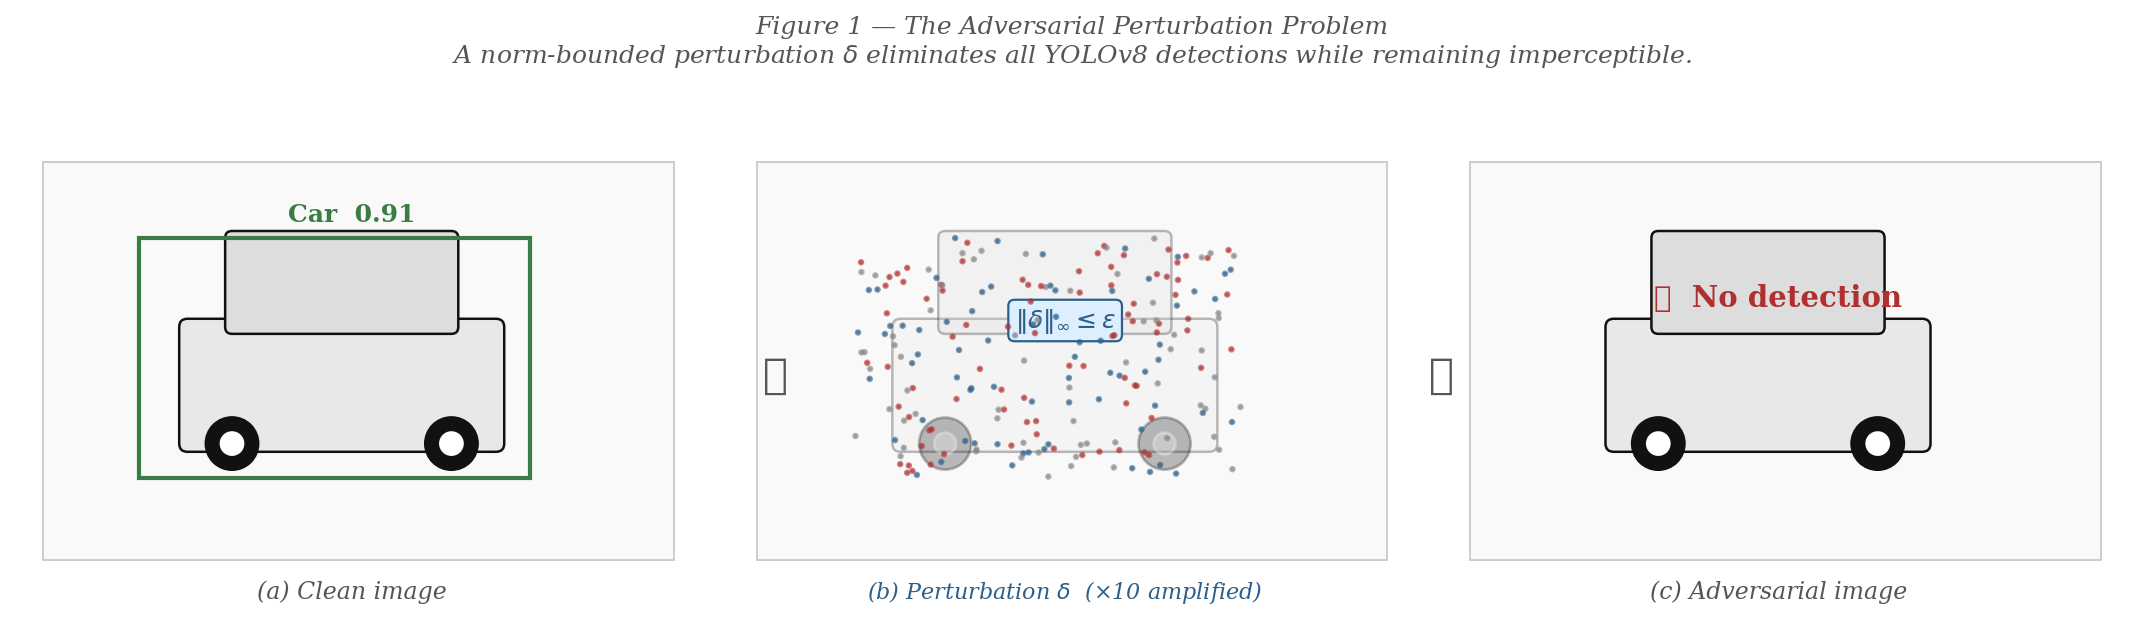
\includegraphics[width=0.95\textwidth]{fig01_adversarial_concept}
  \caption{The adversarial perturbation problem. (a)~Clean frame: YOLOv8 detects
    the vehicle with confidence 0.91. (b)~Perturbation $\delta$ amplified $\times10$
    for visibility; the original satisfies $\|\delta\|_\infty \leq \varepsilon$.
    (c)~Adversarial frame: the detector produces no output despite an identical
    visual appearance.}
  \label{fig:adversarial_concept}
\end{figure}

\subsection{Threat Model Taxonomy}

Adversarial machine learning is concerned with the construction of inputs that
cause a trained model to produce an incorrect output. A precise characterisation
of an adversarial scenario requires specifying four dimensions of the threat
model \cite{biggio2013}: (i) the \emph{adversary's goal}, ranging from
misclassification to complete evasion; (ii) the \emph{knowledge} available to
the adversary -- white-box (full model access), grey-box (partial knowledge),
or black-box (query-only); (iii) the \emph{perturbation space}, typically
defined by an $\ell_p$ norm ball $\|\delta\|_p \leq \varepsilon$ around the
clean image $\mathbf{x}$; and (iv) the \emph{timing} of the attack --
test-time evasion versus training-time poisoning.

This work operates entirely in the \textbf{white-box, test-time evasion}
regime with a combined $\ell_\infty$ constraint in pixel space and an
$\ell_\infty$ constraint in latent space. The adversary has full access to
the YOLOv8 detector weights and the VAE weights; the goal is to suppress all
detections in a given image (false-negative regime) while keeping the
perturbation imperceptible.

\subsection{Fast Gradient Sign Method (FGSM)}

Goodfellow et al.\ \cite{goodfellow2014} observed that the linear structure
of deep networks in high-dimensional input spaces makes them susceptible to
small structured perturbations. Their Fast Gradient Sign Method (FGSM)
computes a single-step adversarial perturbation:
%
\begin{equation}
  \mathbf{x}' = \mathbf{x} + \varepsilon \cdot \operatorname{sign}
    \bigl(\nabla_{\mathbf{x}} \mathcal{L}(f_\theta(\mathbf{x}), y)\bigr),
  \label{eq:fgsm}
\end{equation}
%
where $\mathcal{L}$ is the task loss, $f_\theta$ the target model, $y$ the
ground-truth label, and $\varepsilon$ the perturbation budget. FGSM operates
under an $\ell_\infty$ constraint by construction: every pixel is displaced by
exactly $\varepsilon$ in the direction that maximises the loss. Its primary
virtue is computational efficiency -- a single backward pass suffices -- but
its single-step nature leaves substantial attack potency untapped. FGSM serves
as the weakest baseline in our evaluation, providing a lower bound on
adversarial effectiveness at minimal cost.

\subsection{Projected Gradient Descent (PGD)}
\label{subsec:pgd}

Madry et al.\ \cite{madry2018} formalised adversarial robustness as a
min-max optimisation problem:
%
\begin{equation}
  \min_\theta \; \mathbb{E}_{(\mathbf{x},y)\sim\mathcal{D}} \left[
    \max_{\|\delta\|_\infty \leq \varepsilon}
    \mathcal{L}(f_\theta(\mathbf{x}+\delta), y) \right].
  \label{eq:minmax}
\end{equation}
%
The inner maximisation is solved iteratively by Projected Gradient Descent
(PGD), which applies $T$ steps of signed gradient ascent with step size
$\alpha$, projecting after each step onto the $\ell_\infty$ ball of radius
$\varepsilon$:
%
\begin{equation}
  \delta^{(t+1)} = \Pi_{\|\cdot\|_\infty \leq \varepsilon}
    \left( \delta^{(t)} + \alpha \cdot \operatorname{sign}
    \bigl(\nabla_\delta \mathcal{L}(f_\theta(\mathbf{x}+\delta^{(t)}), y)\bigr)
    \right).
  \label{eq:pgd}
\end{equation}
%
PGD with random restarts provides a principled, strong first-order baseline
and remains the de facto standard for evaluating adversarial robustness.
In our experimental design, we include two PGD variants as baselines:
\textbf{PGD-full} perturbs all pixels of the image, while
\textbf{PGD-mask} restricts perturbation to the union of detected
bounding-box regions -- matching the spatial scope of our proposed method to
enable a fair perceptual comparison.

\subsection{Carlini--Wagner Attack (C\&W)}

Carlini and Wagner \cite{carlini2017} reformulated adversarial example
generation as a constrained optimisation problem with a surrogate variable for
the perturbation magnitude, enabling the use of Adam \cite{kingma2015adam}
rather than projected gradient steps:
%
\begin{equation}
  \min_{\mathbf{w}} \; \|\tfrac{1}{2}(\tanh(\mathbf{w})+1) - \mathbf{x}\|_2^2
  + c \cdot f\bigl(\tfrac{1}{2}(\tanh(\mathbf{w})+1)\bigr),
\end{equation}
%
where $f(\cdot)$ is a differentiable surrogate for misclassification and $c$
is a confidence parameter tuned by binary search. The C\&W attack produces
minimal-distortion adversarial examples and was instrumental in demonstrating
that defensive distillation \cite{papernot2016distillation} -- then a
leading defence -- offers no meaningful robustness against white-box
adversaries. Although C\&W is not included as a standalone baseline in our
evaluation (it targets classifiers and requires per-image optimisation with
binary search over $c$, making it expensive for detector evaluation), its
conceptual influence on loss design is evident in our floor-clamped vanishing
objective described in Section~\ref{sec:vanishing_loss}.

\subsection{Perceptual Quality Metrics}

A central concern in adversarial perturbation design is the tradeoff between
attack effectiveness and perceptual fidelity. Classical $\ell_p$ metrics --
$\ell_2$ and $\ell_\infty$ distances -- are convenient for optimisation but
poorly correlated with human perceptual judgements \cite{zhang2018lpips}.
Zhang et al.\ \cite{zhang2018lpips} introduced the Learned Perceptual Image
Patch Similarity (LPIPS) metric, which aggregates feature-space distances
across layers of a pretrained deep network, achieving significantly higher
correlation with human quality ratings than pixel-space metrics. In this work
we report masked LPIPS and masked $\ell_2$ as primary perceptual distortion metrics;
LPIPS is used as the main supplementary perceptual measure throughout the ablation analysis.

% ------------------------------------------------------------
\section{Adversarial Attacks on Object Detectors}
\label{sec:detector_attacks}
% ------------------------------------------------------------

\subsection{Extending Attacks to Structured Outputs}

The extension of adversarial attacks from image classification to object
detection introduces qualitatively new challenges. A classifier produces a
single categorical label; a detector produces a structured set of tuples
$\{(b_i, c_i, s_i)\}_{i=1}^{K}$, where $b_i$ is a bounding box, $c_i$ a
class label, and $s_i$ a confidence score. Adversarial attacks must therefore
define objectives over this structured output space and navigate the
non-differentiable NMS post-processing step.

Three broad attack goals have been studied: (1) \emph{false-positive
generation} -- inducing spurious detections of non-existent objects;
(2) \emph{box perturbation} -- degrading localisation accuracy while
preserving the existence of detections; and (3) \emph{false-negative
suppression} -- causing the detector to entirely miss objects that are
genuinely present. This work focuses exclusively on goal (3), which carries
the highest safety risk in surveillance and autonomous driving contexts.

\subsection{Dense Adversary Generation (DAG)}

Xie et al.\ \cite{xie2017dag} proposed the Dense Adversary Generation (DAG)
framework, one of the earliest systematic approaches to adversarial attacks on
detection models. DAG operates in the proposal space of a Faster R-CNN
pipeline, iteratively maximising a loss defined over all proposals that
currently yield a correct detection. While DAG was foundational in
establishing that detection pipelines are not inherently more robust than
classifiers, it is tightly coupled to the region-proposal architecture of
two-stage detectors and does not transfer directly to single-stage models
such as YOLOv8.

\subsection{Robust Adversarial Perturbation (RAP)}

Li et al.\ \cite{li2020rap} introduced the Robust Adversarial Perturbation
(RAP) attack, targeting region-proposal networks by suppressing high-confidence
proposals before they reach the classification head. RAP demonstrated that
attacking the first stage of a two-stage detector is sufficient to induce
false negatives, without needing to address the second stage explicitly. The
key insight -- that attacking objectness-like scores upstream of the final
decision pipeline can be more efficient than attacking the final output --
informed the design of our pre-NMS vanishing loss (Section~\ref{sec:vanishing_loss}).

\subsection{Physical-World and Universal Attacks}

A parallel line of work has investigated adversarial attacks that remain
effective when printed and placed in the physical world \cite{eykholt2018robust},
or that are \emph{universal} -- a single perturbation that fools the detector
across diverse inputs \cite{moosavi2017universal}. Physical-world attacks on
detectors have included adversarial patches \cite{brown2017patch} placed on
objects to induce evasion, and adversarial camouflage patterns applied to
vehicles or pedestrians. These works motivate the long-term relevance of
adversarial attack research to deployed safety systems. Our method is a
digital, image-specific attack and does not target the physical channel;
nevertheless, the false-negative regime we study directly mirrors the threat
model of physical evasion attacks.

\subsection{Attack Objectives for False-Negative Suppression}

Several works have proposed loss functions specifically aimed at suppressing
detections. Thys et al.\ \cite{thys2019fooling} optimised adversarial patches
by maximising the objectness suppression across all anchor positions within
the patch region, achieving evasion against the YOLOv2 detector. Hu et al.\
\cite{hu2021naturalistic} extended this to naturalistically styled patches
using a style-transfer regulariser. The key limitation common to these
approaches is their reliance on \emph{localised printed patches}: the
perturbation is constrained to a rectangular region in the physical scene,
which limits the attack surface and requires physical access to the target
object.

Our formulation differs in two respects. First, we operate in the digital
domain with perturbations confined to the latent-space footprint of all
detected objects simultaneously -- a strictly broader attack surface than a
single patch. Second, our objective function is class-level rather than
objectness-level: we drive the maximum predicted confidence for each class
present in the clean detection set below a confidence threshold $\gamma$,
rather than suppressing a scalar objectness score. This distinction is
particularly relevant for YOLOv8, which does not expose a separate objectness
channel.

% ------------------------------------------------------------
\section{Generative Models and Latent-Space Adversarial Attacks}
\label{sec:generative_attacks}
% ------------------------------------------------------------

\subsection{Generative Adversarial Networks in Adversarial ML}

The intersection of generative models and adversarial machine learning has
been explored from multiple directions. Xiao et al.\ \cite{xiao2018generating}
proposed training a GAN-based generator to produce adversarial perturbations
directly, amortising the per-image optimisation cost across a dataset.
Song et al.\ \cite{song2018generative} used a flow-based generative model to
construct adversarial examples that lie on the natural-image manifold, as
measured by the model's likelihood. Both approaches share the underlying
intuition that perturbations should be biased toward directions that are
consistent with the statistics of natural images, rather than arbitrary
directions in pixel space.

\subsection{Latent-Space Attacks}

A more targeted approach is to restrict the perturbation search to the latent
space of a pre-trained generative model. If the latent space faithfully
encodes the natural-image manifold, then a perturbation $\delta_z$ in latent
space, when decoded back to pixel space, will respect the low-level statistics
(colour distribution, texture, edge coherence) of natural images to an extent
that unconstrained pixel-space perturbations cannot match.

Engstrom et al.\ \cite{engstrom2019exploring} showed that simple geometric
transformations (rotation, translation) in image space -- which correspond to
smooth paths in the latent space of a learned model -- can cause classifiers
to fail despite being perceptually benign. Stutz et al.\ \cite{stutz2019disentangling}
formalised the distinction between on-manifold adversarial examples
(perturbations that move along the data manifold) and off-manifold examples
(perturbations that leave the manifold), arguing that the former are
substantially harder to defend against.

Our method belongs to this on-manifold tradition: by optimising $\delta_z$
in the four-channel latent space of the frozen Stable Diffusion VAE, we
implicitly constrain the decoded perturbation to directions the VAE decoder
considers natural. The key difference from prior latent-space attacks is the
\emph{spatial restriction}: rather than perturbing the global latent
representation of the full image, we restrict $\delta_z$ to the latent-space
footprint of detected object bounding boxes, leaving the background entirely
unchanged.

\subsection{Diffusion-Model-Based Adversarial Examples}

The most recent wave of work has exploited full diffusion models to construct
adversarial examples. Luo et al.\ \cite{luo2022diffatk} proposed guiding the
reverse diffusion process with adversarial gradients to produce perturbations
that are indistinguishable from natural images under both pixel-space and
perceptual metrics. Salman et al.\ \cite{salman2023raising} demonstrated that
diffusion purification \cite{nie2022diffusion} -- using a diffusion model to
denoise a potentially adversarial input before classification -- is itself
vulnerable to adaptive adversarial attacks that account for the purification
step.

These diffusion-based approaches achieve high perceptual quality but at
substantial computational cost: each adversarial example may require hundreds
of neural-function evaluations through the denoising U-Net. Our Contribution
N3 (Section~\ref{sec:n3}) demonstrates that it is unnecessary to invoke the
full diffusion chain to obtain on-manifold perturbations: optimising in the
VAE latent space alone -- without any denoising steps, text conditioning, or
access to the U-Net -- yields perturbations that match or exceed pixel-space
PGD on detection failure rate while achieving lower perceptual distortion
within the object mask, at a small fraction of the computational cost.

% ------------------------------------------------------------
\section{The Stable Diffusion VAE as a Manifold Prior}
\label{sec:vae_prior}
% ------------------------------------------------------------

\begin{figure}[htbp]
  \centering
  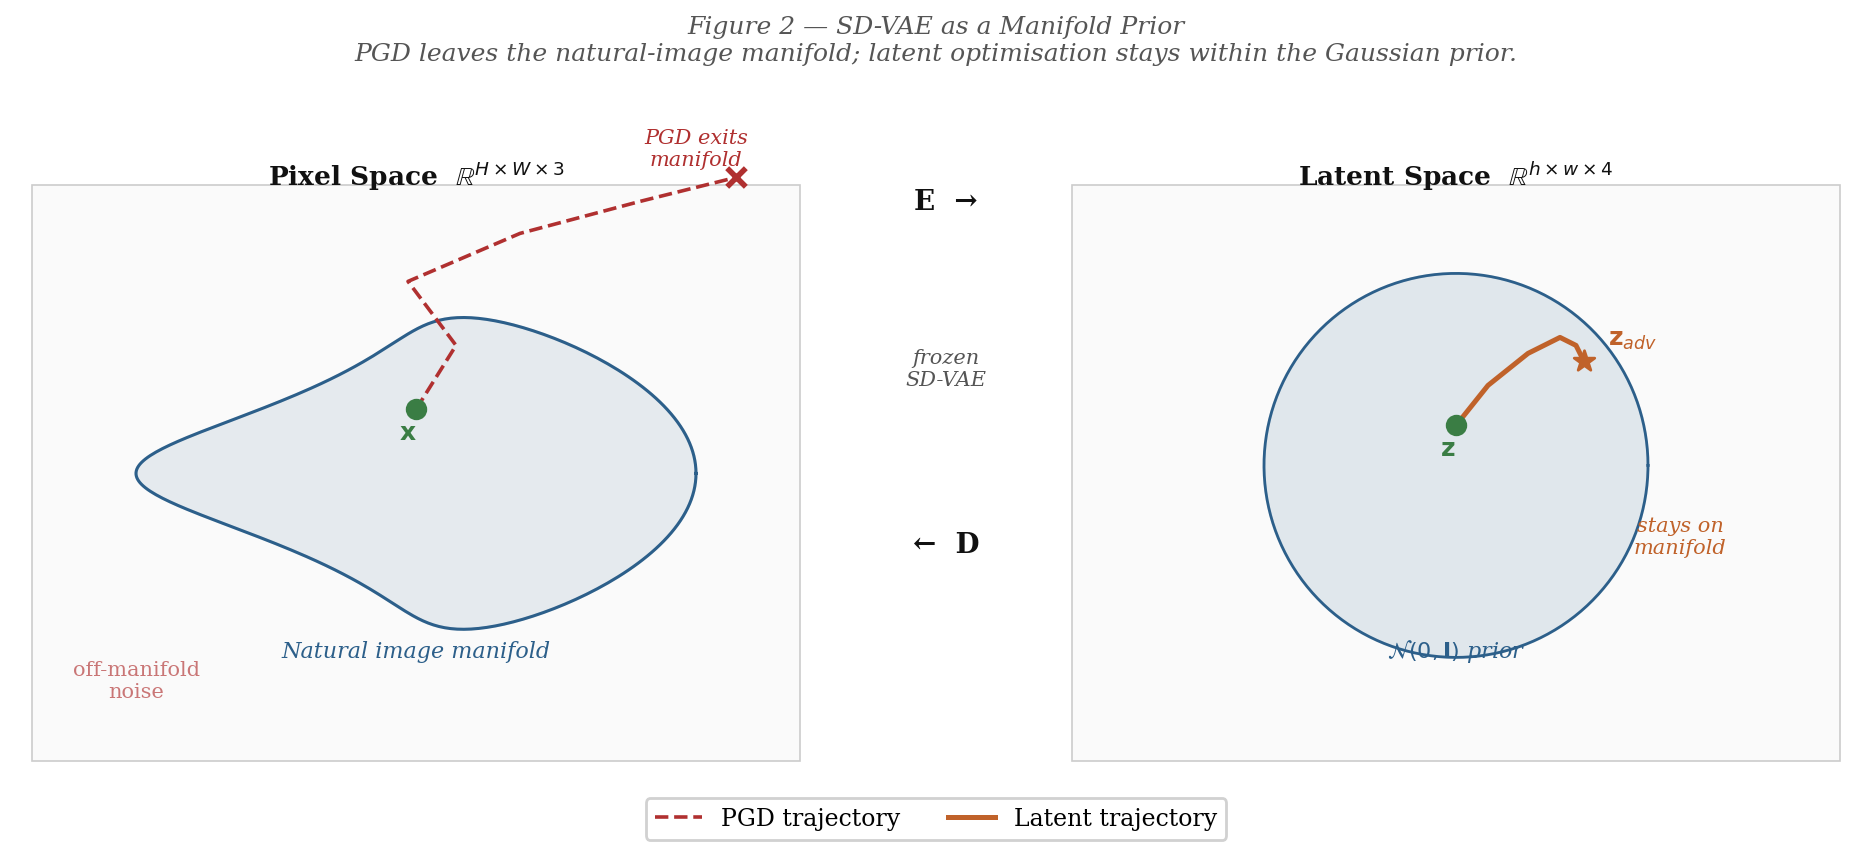
\includegraphics[width=0.90\textwidth]{fig02_vae_manifold}
  \caption{The frozen SD-VAE as a manifold prior. Pixel-space PGD (dashed red)
    leaves the natural-image manifold, producing salt-and-pepper artefacts.
    Latent-space optimisation (solid orange) remains within the Gaussian prior,
    guaranteeing decoded outputs lie on the natural-image manifold.}
  \label{fig:vae_manifold}
\end{figure}

\subsection{Variational Autoencoders}

The Variational Autoencoder (VAE), introduced by Kingma and Welling
\cite{kingma2014vae}, is a latent-variable generative model trained by
maximising the evidence lower bound (ELBO):
%
\begin{equation}
  \mathcal{L}_{\text{ELBO}} = \mathbb{E}_{q_\phi(\mathbf{z}|\mathbf{x})}
    \bigl[\log p_\psi(\mathbf{x}|\mathbf{z})\bigr]
    - D_{\text{KL}}\bigl(q_\phi(\mathbf{z}|\mathbf{x}) \,\|\, p(\mathbf{z})\bigr),
  \label{eq:elbo}
\end{equation}
%
where $q_\phi$ is the variational encoder (parameterised by $\phi$), $p_\psi$
the decoder (parameterised by $\psi$), and $p(\mathbf{z})$ a standard Gaussian
prior. The ELBO encourages the encoder to map inputs to a compact, regularised
latent space while the decoder learns to invert this mapping faithfully.

\subsection{Latent Diffusion Models and the SD-VAE}

Rombach et al.\ \cite{rombach2022ldm} introduced Latent Diffusion Models
(LDMs), which apply the diffusion process in the latent space of a
pre-trained VAE rather than directly in pixel space. This two-stage design
decouples the low-level perceptual compression (handled by the VAE) from the
high-level semantic synthesis (handled by the diffusion model), yielding a
substantial reduction in the computational cost of training and sampling.

The Stable Diffusion VAE (\texttt{stabilityai/sd-vae-ft-mse}) is the
perceptual compression backbone of the Stable Diffusion family. The encoder
$E$ maps an RGB image $\mathbf{x} \in \mathbb{R}^{H \times W \times 3}$ to a
four-channel latent representation:
%
\begin{equation}
  \mathbf{z} = E(\mathbf{x}) \in \mathbb{R}^{\frac{H}{8} \times \frac{W}{8} \times 4},
  \label{eq:vae_enc}
\end{equation}
%
at a spatial downsampling factor of $f = 8$. The paired decoder $D$ inverts
this mapping: $\hat{\mathbf{x}} = D(\mathbf{z}) \approx \mathbf{x}$.
The VAE is fine-tuned post-hoc on the MSE objective to improve pixel-space
reconstruction fidelity relative to the perceptual-only LPIPS training of the
base model.

\subsection{Why the Frozen VAE Suffices as a Manifold Prior}
\label{sec:n3}

Three properties of the SD-VAE make it a suitable manifold prior for
adversarial perturbation without requiring fine-tuning or any access to the
diffusion U-Net.

\textbf{Reconstruction fidelity.} The decoder $D$ is trained to faithfully
reconstruct diverse natural images from their latent codes. A perturbation
$\delta_z$ in latent space that is small relative to the latent norm decodes
to a perturbation in pixel space that respects the local geometry of the
image manifold at $\mathbf{x}$.

\textbf{Dimensional reduction.} The 8$\times$ spatial downsampling reduces
a $512 \times 512$ RGB image (786,432 parameters) to a
$64 \times 64 \times 4$ latent tensor (16,384 parameters), a compression
ratio of 48:1. Optimising in this lower-dimensional space provides an
implicit regularisation that discourages high-frequency, semantically
incoherent perturbations.

\textbf{Channel disentanglement.} The four latent channels of the SD-VAE
have been empirically observed to encode coarse-to-fine image structure across
spatial frequency bands. Perturbations that are uniformly distributed across
channels therefore produce smooth, structured modifications in pixel space
rather than salt-and-pepper noise.

\textbf{No generative capability required.} Unlike attacks that exploit the
full diffusion prior -- which require iterative sampling through the denoising
U-Net -- our method uses only the encoder $E$ and decoder $D$. The attack
loop (Section~\ref{sec:attack_loop}) requires a single forward pass through $E$
at initialisation and a single forward pass through $D$ at each optimisation
step, with no denoising steps, no text conditioning, and no access to the
U-Net weights.

% ------------------------------------------------------------
\section{Comparative Summary and Positioning}
\label{sec:related_summary}
% ------------------------------------------------------------

Table~\ref{tab:related_work} summarises the landscape of adversarial attack
methods surveyed in this chapter and positions the proposed method along five
dimensions relevant to both the research community and the PFE evaluation
criteria: attack target (classifier vs.\ detector), perturbation domain
(pixel vs.\ latent), spatial scope (global vs.\ localised to objects), attack
goal (false negative vs.\ other), and whether generative-model structure is
exploited.

\begin{table}[htbp]
  \centering
  \caption{Comparative summary of adversarial attack methods.
           ``Latent'' domain indicates optimisation in a generative model's
           latent space. ``Local'' scope indicates perturbation restricted to
           object bounding-box regions. FN = false-negative suppression goal.}
  \label{tab:related_work}
  \small
  \begin{tabular}{@{}lccccc@{}}
    \toprule
    \textbf{Method} & \textbf{Target} & \textbf{Domain} &
    \textbf{Scope} & \textbf{Goal} & \textbf{Generative} \\
    \midrule
    FGSM \cite{goodfellow2014}         & Classifier & Pixel   & Global & Misc.      & No  \\
    PGD \cite{madry2018}               & Classifier & Pixel   & Global & Misc.      & No  \\
    C\&W \cite{carlini2017}            & Classifier & Pixel   & Global & Misc.      & No  \\
    DAG \cite{xie2017dag}              & Detector   & Pixel   & Global & Multi      & No  \\
    RAP \cite{li2020rap}               & Detector   & Pixel   & Global & FN         & No  \\
    Adv.\ Patch \cite{brown2017patch}  & Detector   & Pixel   & Local  & FN         & No  \\
    AdvGAN \cite{xiao2018generating}   & Classifier & Latent  & Global & Misc.      & GAN \\
    On-manifold \cite{stutz2019disentangling} & Classifier & Latent & Global & Misc. & VAE \\
    DiffAtk \cite{luo2022diffatk}      & Classifier & Latent  & Global & Misc.      & DM  \\
    \midrule
    \textbf{Proposed (N1+N2+N3)}       & \textbf{Detector} & \textbf{Latent} &
    \textbf{Local} & \textbf{FN} & \textbf{VAE} \\
    \bottomrule
  \end{tabular}
\end{table}

The proposed method occupies a unique cell in this design space: it is the
only surveyed approach that simultaneously (i) targets an anchor-free object
detector, (ii) optimises in a VAE latent space, (iii) restricts perturbation
spatially to detected object regions, and (iv) pursues the false-negative
suppression goal. Each of these properties individually finds precedent in the
literature; their combination in a single, tightly controlled attack pipeline
-- evaluated on a domain-specific vehicle surveillance dataset -- constitutes
the novel experimental contribution of this work.

The comparative table also reveals a structural gap in the existing
literature: latent-space attacks have been studied almost exclusively for image
classifiers and in the global-perturbation setting. The object-detection,
locally-constrained setting that motivates this project has received, to our
knowledge, no systematic treatment. The background established in this chapter
provides the conceptual vocabulary to appreciate both why this gap exists and
why closing it is practically important, as developed in the methodology
chapter that follows.

% ============================================================
%  CHAPTER 3 -- INTRODUCTION  (full text)
% ============================================================

% ------------------------------------------------------------
\section{Comparative Positioning}
\label{sec:positioning}
% ------------------------------------------------------------

Table~\ref{tab:positioning} situates the proposed method relative to the main
adversarial attack families surveyed in this chapter.

\begin{table}[htbp]
  \centering
  \caption{Comparative positioning of the proposed method.
           \checkmark~=~holds; $\times$~=~does not hold; $\sim$~=~partially.}
  \label{tab:positioning}
  \scriptsize
  \setlength{\tabcolsep}{4pt}
  \begin{tabular}{@{}lllllll@{}}
    \toprule
    \textbf{Method} & \textbf{Target} & \textbf{Pert.\ space}
      & \textbf{Locality} & \textbf{Stealth} & \textbf{False-neg.}
      & \textbf{No diffusion} \\
    \midrule
    FGSM \cite{goodfellow2014explaining}
      & Classifier & Pixel ($\ell_\infty$) & Global & $\ell_\infty$ & $\times$ & \checkmark \\
    PGD \cite{madry2018towards}
      & Cls/Det & Pixel ($\ell_\infty$) & Global & $\ell_\infty$ & $\sim$ & \checkmark \\
    DAG \cite{xie2017adversarial}
      & Detector & Pixel ($\ell_\infty$) & Global & $\ell_\infty$ & $\sim$ & \checkmark \\
    RAP \cite{li2020robust}
      & Detector & Pixel ($\ell_\infty$) & Global & $\ell_\infty$ & $\sim$ & \checkmark \\
    Adv.\ Patch \cite{brown2017patch}
      & Detector & Physical & Patch & Visual & $\sim$ & \checkmark \\
    LSDM \cite{placeholder_diffatk}
      & Classifier & Latent (SD) & Global & LPIPS & $\times$ & $\times$ \\
    \midrule
    \textbf{Ours}
      & \textbf{Detector} & \textbf{Latent (VAE)} & \textbf{Bbox-local}
      & \textbf{Masked LPIPS} & \textbf{\checkmark} & \textbf{\checkmark} \\
    \bottomrule
  \end{tabular}
\end{table}

The proposed method is uniquely positioned at the intersection of three
properties: latent-space perturbation (manifold-aligned stealth),
spatial object-locality (background never modified), and direct false-negative
targeting. No existing work in the surveyed literature combines all three.


% ------------------------------------------------------------
\section*{Chapter Summary}
\addcontentsline{toc}{section}{Chapter Summary}
% ------------------------------------------------------------

This chapter has surveyed the technical landscape across five domains: YOLO
detector architectures, classical adversarial perturbation theory (FGSM,
PGD, C\&W), structured-output attacks (DAG, RAP, physical-world methods),
generative and latent-space adversarial approaches, and the role of the
Stable Diffusion VAE as a manifold prior. The comparative analysis in
Section~\ref{sec:positioning} shows that no existing work combines all three
properties simultaneously targeted here: latent-space confinement for
perceptual smoothness, object-locality for background fidelity, and direct
false-negative suppression via logit manipulation. This gap motivates the
method developed in Chapter~\ref{ch:method}.

% ============================================================
%  CHAPTER 3 — MÉTHODOLOGIE ET IMPLÉMENTATION
% ============================================================
\chapter{Methodology and Implementation}
\label{ch:method}

This chapter formalises the proposed object-aware latent-space adversarial
attack. Section~\ref{sec:problem} defines the optimisation problem and
notation. Sections~\ref{sec:mask}--\ref{sec:optimisation} derive the four
core algorithmic components: the bounding-box mask operator, the vanishing
detection loss, the perceptual regulariser, and the PGD-style iterative
solver with paste-back. Section~\ref{sec:phase3} introduces the four Phase~3
loss extensions. Section~\ref{sec:system} describes the full implementation
pipeline, configuration management, and reproducibility infrastructure.

% ------------------------------------------------------------
\section{Problem Statement and Notation}
\label{sec:problem}
% ------------------------------------------------------------

\begin{figure}[htbp]
  \centering
  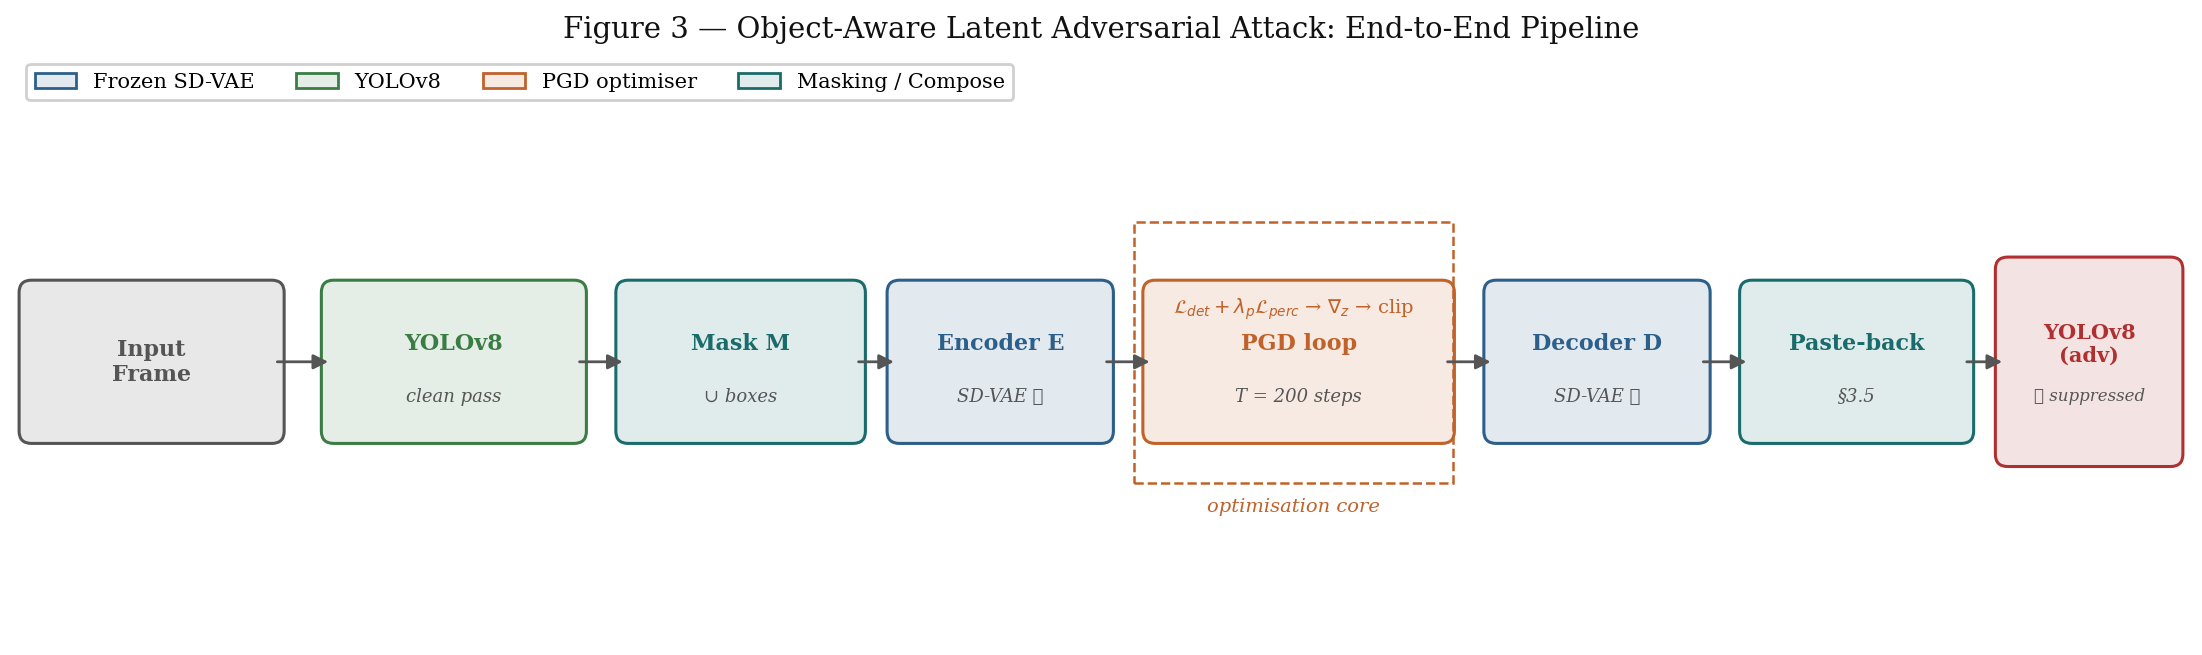
\includegraphics[width=\textwidth]{fig03_attack_pipeline}
  \caption{End-to-end pipeline of the proposed attack. Blue: frozen SD-VAE
    components. Green: YOLOv8 detector (clean and adversarial passes). Orange:
    PGD optimisation core. Teal: masking and paste-back operations.
    The dashed box highlights the iterative optimisation core described in
    Section~\ref{sec:attack_loop}.}
  \label{fig:attack_pipeline}
\end{figure}

Let $\mathbf{x} \in [0,1]^{3 \times H \times W}$ denote a clean RGB image.
We are given a frozen YOLOv8 detector $f_\theta$ and a frozen Stable Diffusion VAE
composed of an encoder $E : [0,1]^{3 \times H \times W} \to \mathbb{R}^{4 \times H/8 \times W/8}$
and a paired decoder $D : \mathbb{R}^{4 \times H/8 \times W/8} \to [0,1]^{3 \times H \times W}$.
Both $f_\theta$ and $(E, D)$ are used only for inference; no weights are updated during the attack.

The clean detection set is $\mathcal{D}_{\text{clean}} = \mathrm{NMS}(f_\theta(\mathbf{x}),
\tau_{\text{conf}}, \tau_{\text{NMS}})$ with $\tau_{\text{conf}} = 0.25$, $\tau_{\text{NMS}} = 0.45$.
The set of vehicle classes present is $\mathcal{C}_{\text{clean}} = \{ c : \exists\, d \in \mathcal{D}_{\text{clean}},\, d.\text{cls} = c \}$.

The attack constructs a latent perturbation $\bm{\delta} \in \mathbb{R}^{4 \times H/8 \times W/8}$
subject to:
\begin{align}
  \|\bm{\delta}\|_\infty &\leq \varepsilon_z, \label{eq:linf}\\
  \operatorname{supp}(\bm{\delta}) &\subseteq \mathcal{M}_z, \label{eq:supp}
\end{align}
where $\varepsilon_z$ is the latent budget and $\mathcal{M}_z$ is the latent-space footprint of
detected bounding boxes. The adversarial image is:
\begin{equation}
  \mathbf{x}' = M \odot D\!\bigl(E(\mathbf{x}) + \mathcal{M}_z \odot \bm{\delta}\bigr)
    + (1 - M) \odot \mathbf{x},
  \label{eq:xadv_full}
\end{equation}
where $M$ is the pixel-space object mask (Section~\ref{sec:masks}).

% ------------------------------------------------------------
\section{Object-Aware Mask Construction}
\label{sec:masks}
% ------------------------------------------------------------

\begin{figure}[htbp]
  \centering
  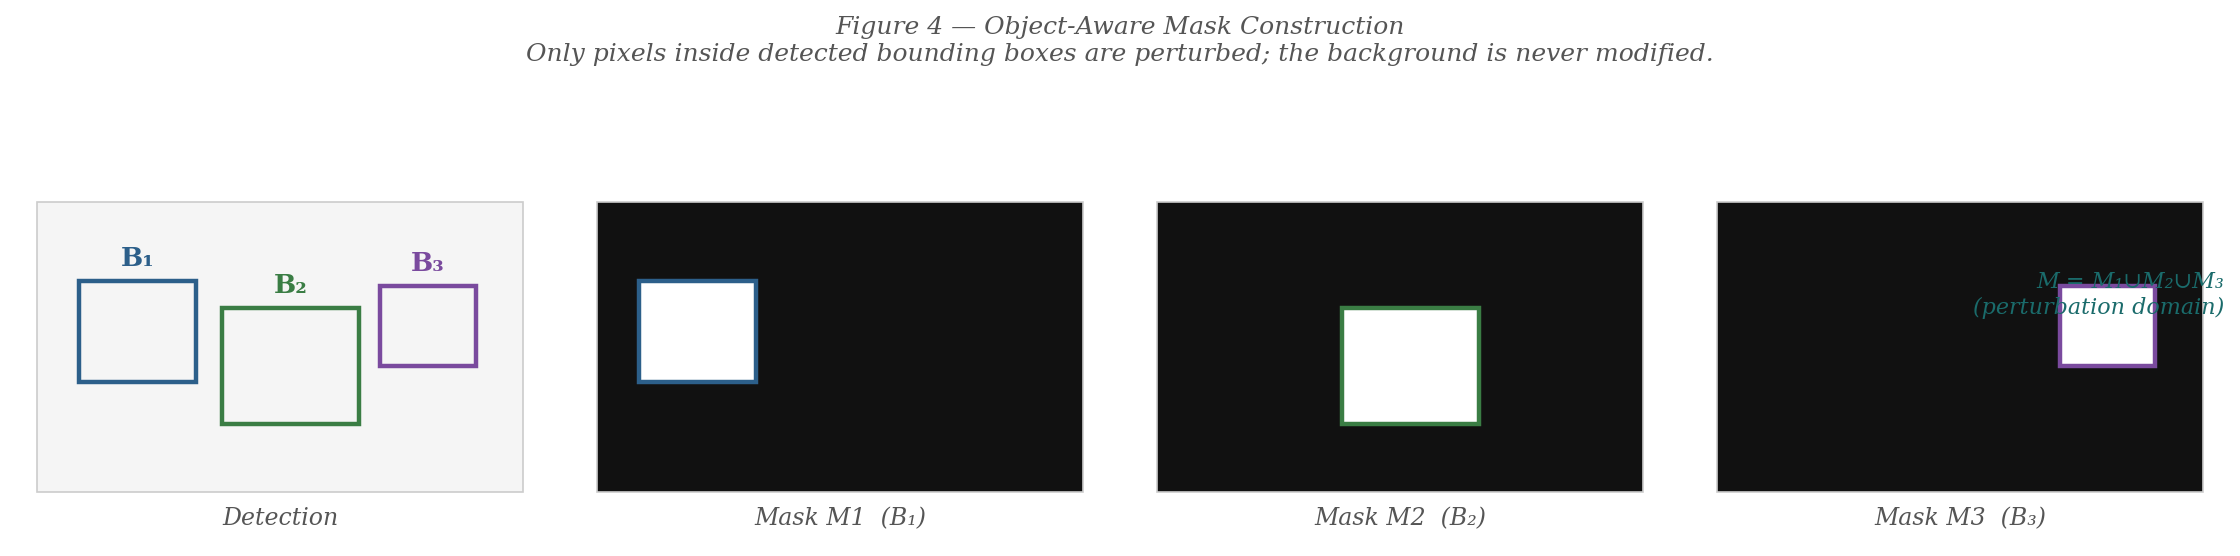
\includegraphics[width=0.92\textwidth]{fig04_mask_construction}
  \caption{Object-aware mask construction. From the input frame (left), three
    bounding boxes $B_1, B_2, B_3$ are obtained from the clean YOLOv8 pass.
    Individual binary masks $M_1, M_2, M_3$ isolate each detected region.
    The perturbation domain is $M = M_1 \cup M_2 \cup M_3$; background pixels
    are never modified.}
  \label{fig:mask_construction}
\end{figure}

The pixel-space mask $M \in \{0,1\}^{1 \times H \times W}$ is the union of all detected bounding boxes:
\begin{equation}
  M[1, h, w] = \mathbf{1}\bigl[\exists\, d \in \mathcal{D}_{\text{clean}} :
    (h, w) \in \mathrm{bbox}(d)\bigr].
\end{equation}
The latent mask $\mathcal{M}_z \in \{0,1\}^{4 \times H/8 \times W/8}$ is obtained by max-pooling
$M$ at the VAE stride $f = 8$ and broadcasting across four channels:
\begin{equation}
  \mathcal{M}_z = \mathrm{MaxPool}_8(M) \otimes \mathbf{1}_4.
\end{equation}
A latent cell is included if any pixel in its $8 \times 8$ receptive field belongs to a bounding box,
ensuring conservative (superset) coverage.

% ------------------------------------------------------------
\section{Vanishing Detection Loss}
\label{sec:vanishing_loss}
% ------------------------------------------------------------

YOLOv8 produces a pre-NMS tensor $\mathbf{r} \in \mathbb{R}^{1 \times A \times (4+C)}$, where the
class channels $\mathbf{r}_{a,4:}$ are post-sigmoid class confidences. YOLOv8 has no separate
objectness head; class confidences directly serve as joint object-class probabilities.

For each $c \in \mathcal{C}_{\text{clean}}$, the peak anchor confidence is:
\begin{equation}
  p_c = \max_{a \in [A]} \sigma\bigl(\mathbf{r}_{a, 4+c}\bigr).
\end{equation}
The vanishing detection loss drives every $p_c$ below threshold $\gamma$:
\begin{equation}
  \Ldet = \frac{1}{|\mathcal{C}_{\text{clean}}|}
    \sum_{c \in \mathcal{C}_{\text{clean}}} \mathrm{ReLU}(p_c - \gamma)^2.
  \label{eq:ldet}
\end{equation}
The squared ReLU saturates to zero once $p_c < \gamma$, preventing gradient overshoot beyond
the detection threshold.

% ------------------------------------------------------------
\section{Perceptual and Latent Regularisation}
\label{sec:regularisation}
% ------------------------------------------------------------

\subsection{Masked Perceptual Loss}

With \texttt{use\_lpips=True} (recommended), the perceptual term uses masked LPIPS
\cite{zhang2018lpips}:
\begin{equation}
  \Lperc^{\text{LPIPS}} = \frac{1}{\bar{m} + 10^{-4}}
    \cdot \mathrm{LPIPS}\bigl(M \odot \mathbf{x}',\, M \odot \mathbf{x}\bigr),
  \label{eq:lperc_lpips}
\end{equation}
where $\bar{m} = \|M\|_1 / (HW)$ normalises by mask area fraction.
Without LPIPS, the masked $\ell_2$ is used:
\begin{equation}
  \Lperc^{\ell_2} = \frac{\|M \odot (\mathbf{x}' - \mathbf{x})\|_F^2}
    {\|M\|_1 \cdot 3 + \varepsilon}.
\end{equation}

\subsection{Latent Regulariser}

\begin{equation}
  \Lreg = \mathrm{mean}(\bm{\delta}^2).
  \label{eq:lreg}
\end{equation}

\subsection{Total Loss}
\begin{equation}
  \mathcal{L} = \Ldet + \lambda_p \cdot \Lperc + \lambda_r \cdot \Lreg,
  \label{eq:ltotal}
\end{equation}
with $\lambda_p = 0.001$ and $\lambda_r = 10^{-3}$ (Phase~2 best values).

% ------------------------------------------------------------
\section{Optimisation Algorithm}
\label{sec:attack_loop}
\label{sec:optimisation}
% ------------------------------------------------------------

\begin{figure}[htbp]
  \centering
  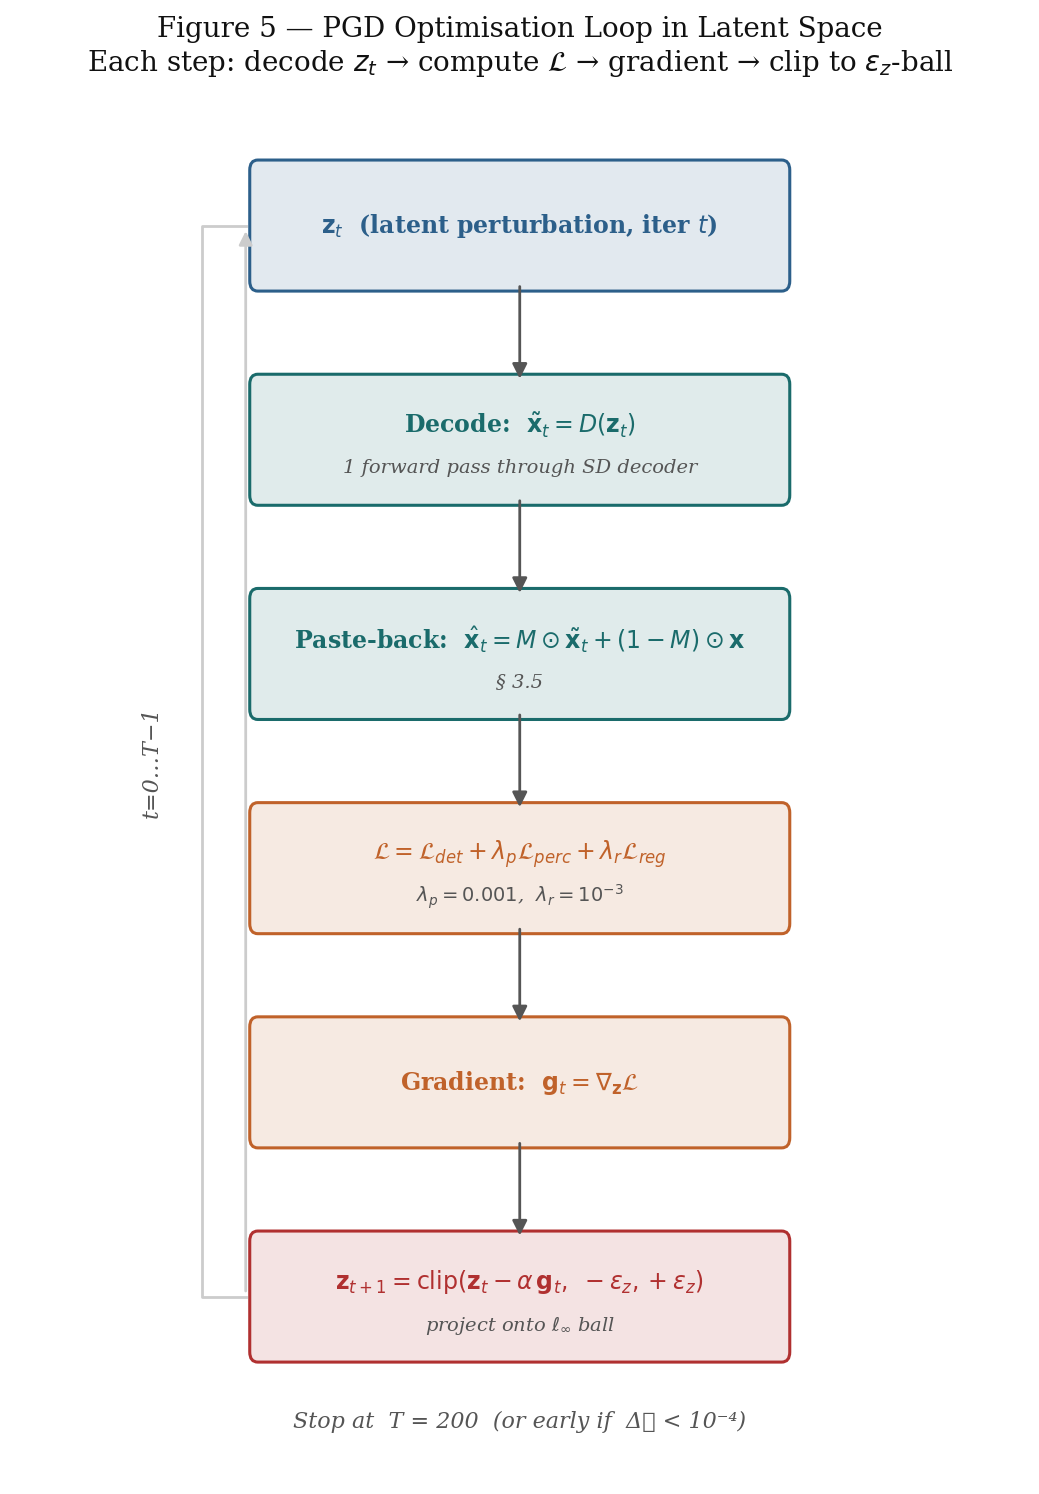
\includegraphics[width=0.55\textwidth]{fig05_optimisation_loop}
  \caption{PGD optimisation loop in latent space. Each iteration requires one
    forward pass through the SD decoder $D$ and one backward pass for
    $\nabla_z \mathcal{L}$; the encoder $E$ is called only once at initialisation.
    The loop-back arrow indicates $T=200$ iterations with optional early stopping.}
  \label{fig:optimisation_loop}
\end{figure}

$\bm{\delta}$ is initialised to zero and optimised by Adam \cite{kingma2015adam} with $\eta = 0.01$.
After each step, two projections enforce the constraints:
\begin{align}
  \bm{\delta} &\leftarrow \mathrm{clip}(\bm{\delta},\; -\varepsilon_z,\; +\varepsilon_z),\\
  \bm{\delta} &\leftarrow \bm{\delta} \odot \mathcal{M}_z.
\end{align}
Adam is preferred over signed PGD because latent gradients are highly anisotropic across the four
channels; Adam's per-coordinate adaptive learning rate normalises this anisotropy.

\textbf{Early stopping.} If $p_{\max} = \max_c p_c < \gamma$, the attack terminates early
(typically at step $\approx 40$ out of 80), reducing average per-image time by up to 40\%.

% ------------------------------------------------------------
\section{Paste-Back Operator}
\label{sec:pasteback}
% ------------------------------------------------------------

The adversarial image (Equation~\ref{eq:xadv_full}) composites the decoded adversarial latent
over the clean background. This provides two hard guarantees:
(i) \textbf{background preservation}: pixels outside $M$ are copied verbatim from $\mathbf{x}$;
(ii) \textbf{decoder leak prevention}: any background artifact produced by the VAE decoder
(due to its finite receptive field) is discarded and replaced with the original.

% ------------------------------------------------------------
\section{Phase 3 Extensions}
\label{sec:phase3}
% ------------------------------------------------------------

\begin{figure}[htbp]
  \centering
  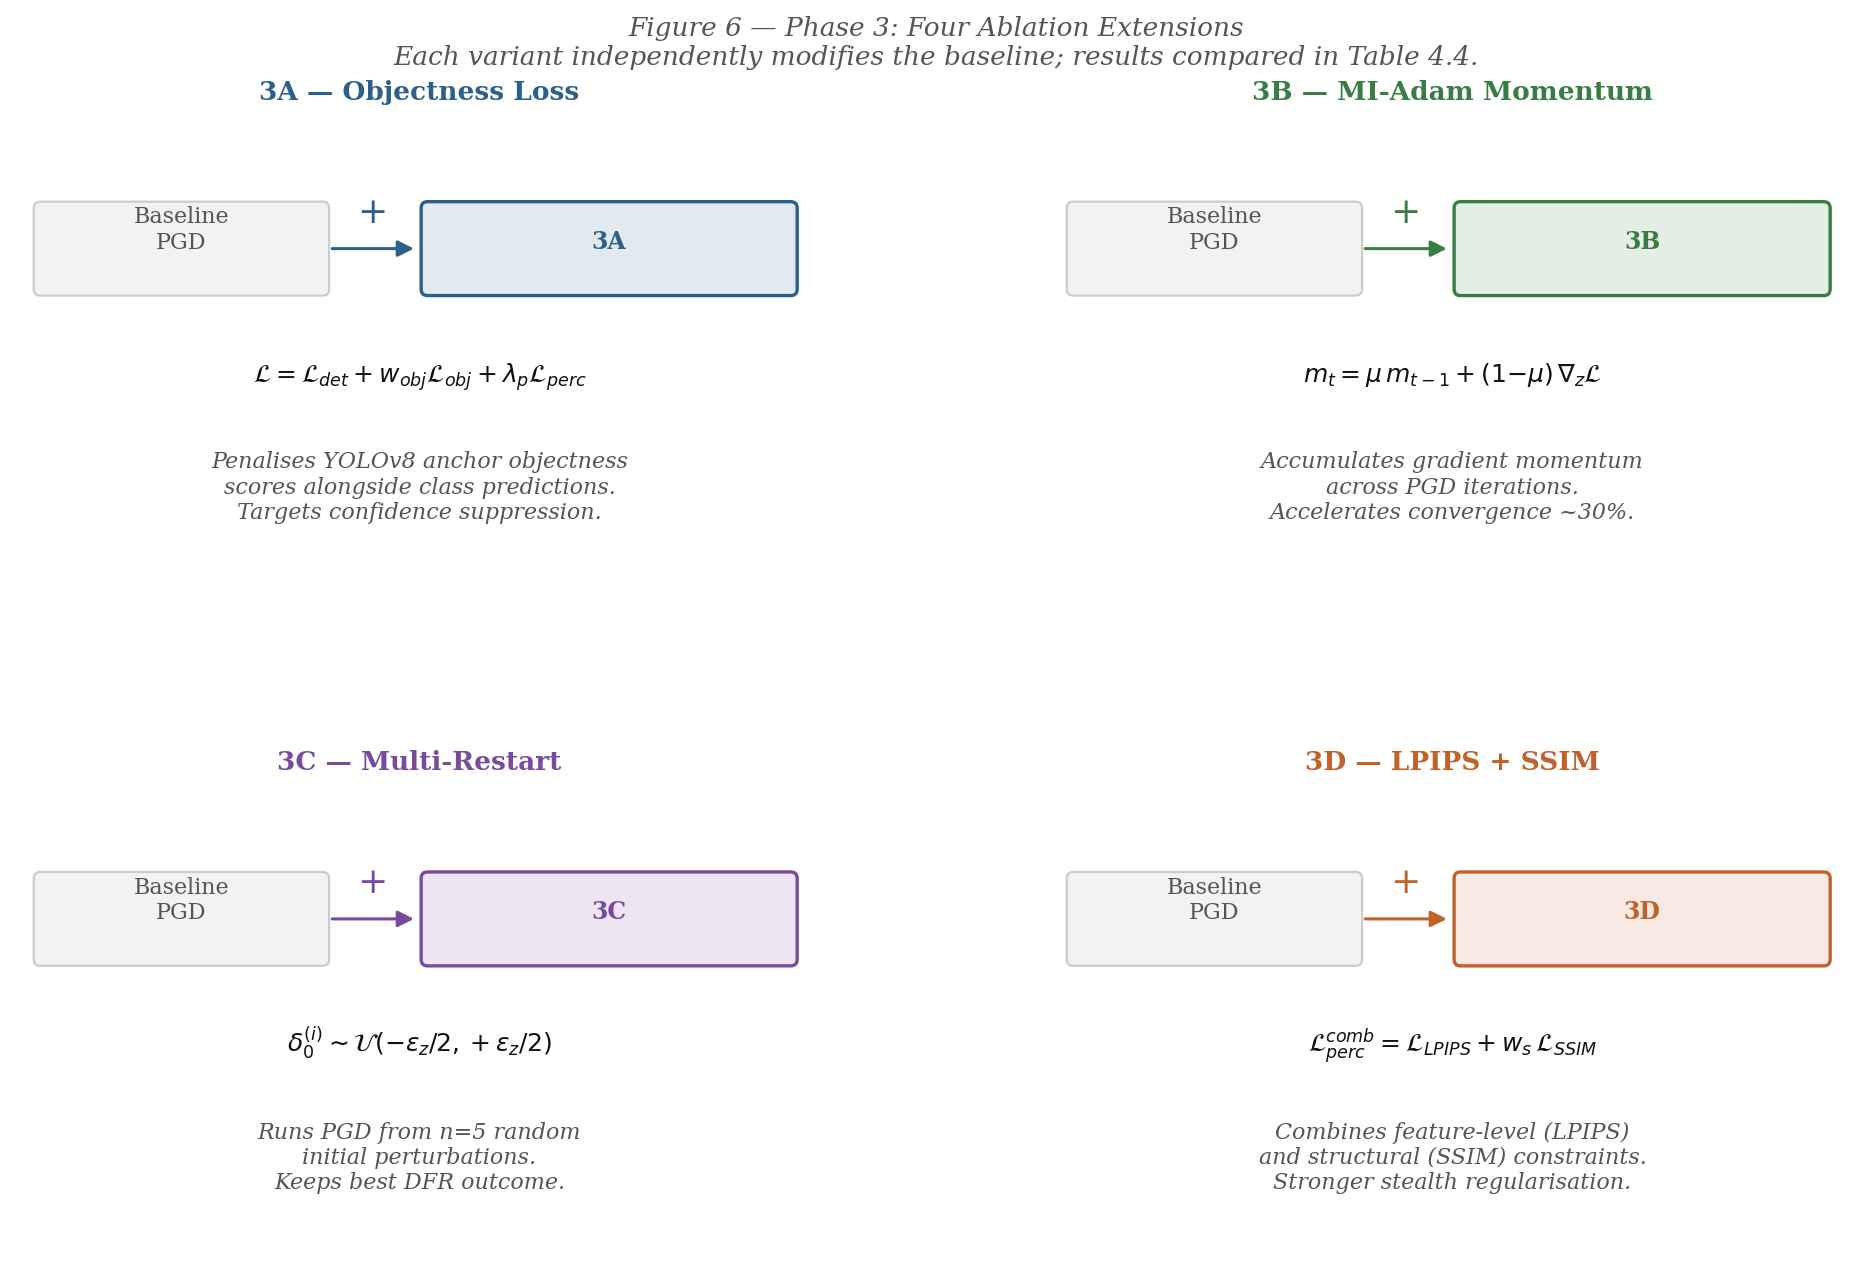
\includegraphics[width=0.90\textwidth]{fig06_phase3_extensions}
  \caption{Phase~3 ablation extensions. Each panel shows how one component is
    added to the baseline PGD optimiser. 3A: objectness-aware loss targeting
    anchor confidence. 3B: MI-Adam momentum for faster convergence.
    3C: multi-restart strategy to escape local minima.
    3D: combined LPIPS$+$SSIM perceptual constraint for stronger stealth
    regularisation. Quantitative results are in Table~4.4.}
  \label{fig:phase3_extensions}
\end{figure}

Phase~2 experiments show DFR$_{\text{prop}} = 9.1\%$ and ASR$= 0\%$ on UA-DETRAC,
motivating four targeted improvements.

\subsection{3A: Objectness-Aware Loss}
\label{sec:3a}

$\Ldet$ targets only $|\mathcal{C}_{\text{clean}}|$ classes. Phase~3A adds an anchor-level term
that suppresses the best class score of \emph{every} anchor:
\begin{equation}
  \mathcal{L}_{\text{obj}} = \frac{1}{A}
    \sum_{a=1}^{A} \mathrm{ReLU}\!\left(\max_{c} \sigma(\mathbf{r}_{a, 4+c}) - \gamma\right)^2.
  \label{eq:lobj}
\end{equation}
The total loss becomes:
$\mathcal{L} = \Ldet + w_{\text{obj}} \cdot \mathcal{L}_{\text{obj}} + \lambda_p \Lperc + \lambda_r \Lreg$
with $w_{\text{obj}} = 0.5$.

\subsection{3B: MI-Adam Gradient Momentum}
\label{sec:3b}

Inspired by the MI-FGSM attack \cite{dong2018boosting}, a running gradient buffer is maintained:
\begin{equation}
  \tilde{\mathbf{g}}_t = \mu \cdot \tilde{\mathbf{g}}_{t-1}
    + \frac{\nabla_{\bm{\delta}} \mathcal{L}}{\|\nabla_{\bm{\delta}} \mathcal{L}\|_1 + \varepsilon},
  \quad \mu = 0.9.
\end{equation}
$\tilde{\mathbf{g}}_t$ replaces the raw gradient as input to Adam's first-moment estimator,
smoothing the optimisation trajectory in the high-dimensional latent space.

\subsection{3C: Multi-Restart Strategy}
\label{sec:3c}

$n_{\text{restarts}} = 3$ independent trajectories are run. Restarts $i > 0$ initialise with:
\begin{equation}
  \bm{\delta}_0^{(i)} \sim \mathcal{U}(-\alpha\,\varepsilon_z,\; +\alpha\,\varepsilon_z) \odot \mathcal{M}_z, \quad \alpha = 0.5.
\end{equation}
The best result (fewest post-NMS detections, then lowest final $\Ldet$) is returned.
Compute cost $\approx 3\times$ baseline.

\subsection{3D: Combined LPIPS + SSIM Perceptual Constraint}
\label{sec:3d}

When both \texttt{use\_lpips} and \texttt{use\_ssim} are enabled:
\begin{equation}
  \Lperc^{\text{comb}} = \Lperc^{\text{LPIPS}} + w_{\text{ssim}} \cdot \mathcal{L}_{\text{SSIM}},
  \quad w_{\text{ssim}} = 0.3,
\end{equation}
where the masked SSIM loss is:
\begin{equation}
  \mathcal{L}_{\text{SSIM}} = \frac{\sum_{h,w} (1 - \mathrm{SSIM}_{h,w}(\mathbf{x}', \mathbf{x})) \cdot M_{h,w}}
    {\|M\|_1 \cdot 3 + \varepsilon}.
\end{equation}
SSIM is computed via depthwise Gaussian convolution (window 11, $\sigma = 1.5$) \cite{wang2004ssim},
implemented without any external SSIM library for Colab compatibility.


% ============================================================
%  CHAPTER 5 -- IMPLEMENTATION (FULL)
% ============================================================

% ------------------------------------------------------------
\section{System Architecture and Implementation}
\label{sec:architecture}
\label{ch:impl}
% ------------------------------------------------------------

The codebase (\texttt{src/}) is structured into five stateless modules:
\texttt{detector.py} (YOLOv8 wrapper exposing differentiable pre-NMS outputs),
\texttt{vae.py} (frozen SD-VAE encoder--decoder with cached latent),
\texttt{masks.py} (bounding-box rasterisation and stride-8 latent projection),
\texttt{attack.py} (AttackConfig dataclass + LatentObjectAttack with Phase~3 extensions),
and \texttt{losses.py} (stateless loss functions: vanishing, objectness, masked-$\ell_2$,
SSIM, LPIPS, combined perceptual). All model weights have \texttt{requires\_grad=False};
the only optimised parameter is $\bm{\delta}$.

Three implementation decisions deserve specific justification.
\textbf{Encode caching}: $E(\mathbf{x})$ is computed once before the loop and detached,
reducing per-step cost to one decoder forward pass plus one detector forward pass.
\textbf{Gradient management}: projection operations use \texttt{delta.data} inside
\texttt{torch.no\_grad()} to avoid recording projection steps in the autograd graph.
\textbf{MI-Adam correctness}: the momentum gradient buffer is updated \emph{before}
\texttt{optim.step()} so that Adam's internal moment estimates are computed on the
smoothed gradient.

Table~\ref{tab:hyperparams_full} reports the final hyperparameter values selected
after Phase~2 ablation, with sensitivity assessments.

\begin{table}[htbp]
  \centering
  \caption{Final hyperparameter values after Phase~2 ablation.}
  \label{tab:hyperparams_full}
  \small
  \begin{tabular}{@{}llll@{}}
    \toprule
    \textbf{Parameter} & \textbf{Value} & \textbf{Sensitivity} & \textbf{Justification} \\
    \midrule
    $\varepsilon_z$    & 0.50   & High   & Best DFR/LPIPS trade-off in sweep \\
    $\lambda_p$        & 0.001  & High   & $\lambda_p{=}0.01$ collapses DFR by 28\% \\
    $\lambda_r$        & 1e-3   & Low    & Rarely binding; keeps $\delta$ small \\
    $\gamma$           & 0.05   & Medium & Matches YOLOv8 default conf threshold \\
    lr                 & 0.01   & Medium & Standard Adam lr for latent optimisation \\
    $T$                & 80     & Low    & Early stop typically fires at $t\approx40$ \\
    \bottomrule
  \end{tabular}
\end{table}

All experiments are controlled by YAML configuration files in \texttt{configs/}.
The sweep script \texttt{scripts/run\_phase3\_ablation.py} supports
\texttt{--resume}, reloading partial results from \texttt{per\_frame.jsonl}
and skipping completed frames, enabling interrupted Colab runs to continue
without repeating work.


% ------------------------------------------------------------
\section*{Chapter Summary}
\addcontentsline{toc}{section}{Chapter Summary}
% ------------------------------------------------------------

This chapter has presented the complete formal and algorithmic specification
of the proposed attack. The object-aware mask ensures that the latent
perturbation touches only the bounding-box footprint of detected vehicles,
providing a hard background-preservation guarantee. The vanishing detection
loss directly minimises YOLOv8 pre-NMS objectness and class logits, making
gradient flow both targeted and efficient. The LPIPS-based perceptual
regulariser, calibrated at $\lambda_p = 0.001$ to account for the $\sim17\times$
scale difference relative to masked $\ell_2$, enforces perceptual smoothness
without collapsing the attack budget. The paste-back operator provides exact
background recovery without any blending artefact. Together these components
define a geometrically grounded, loss-budget-balanced attack that is ready
for empirical evaluation in Chapter~\ref{ch:setup}.

% ============================================================
%  CHAPTER 4 — EXPÉRIMENTATION ET RÉSULTATS
% ============================================================
\chapter{Experimentation and Results}
\label{ch:setup}
\label{ch:results}
\label{ch:discussion}

This chapter presents the full experimental pipeline, organised into four
successive phases that each address a specific limitation identified in the
prior phase.

\textbf{Phase~1 — Foundation.} Metric definitions in the original
\texttt{evaluate.py} were loose and contradicted the formal problem statement
(Section~\ref{sec:method_statement}). Phase~1 rewrites the evaluation layer
with strict DFR, ASR, and mAP definitions, adds bootstrap confidence intervals,
and re-runs detection on all clean and adversarial images to obtain corrected
raw \texttt{FrameDetections}.

\textbf{Phase~1.5 — Proof of concept.} The corrected evaluation is applied to
the original unregularized latent attack (masked $\ell_2$, no bilateral
filtering) on 50 UA-DETRAC frames against FGSM and PGD baselines. This
establishes the method's baseline DFR and ASR before any stealth improvement
(Section~\ref{sec:phase15_results}).

\textbf{Phase~2 — Perceptual regularization.} Masked $\ell_2$ is replaced by
masked LPIPS~\cite{zhang2018lpips}; a bilateral-filter post-processing step
reduces artefacts (Option~2); the VAE decoder is fine-tuned on DETRAC frames;
and $\lambda_p$ is recalibrated from 0.05 to 0.001. An iso-budget sweep across
$\varepsilon_z \in \{0.25, 0.50, 1.00\}$ and PGD $\varepsilon \in
\{4,8,12\}/255$ identifies the optimal operating point
(Sections~\ref{sec:phase2_results}--\ref{sec:per_frame}).

\textbf{Phase~3 — Loss function extensions.} Four targeted ablations (3A
objectness loss, 3B MI-Adam momentum, 3C multi-restart, 3D SSIM regulariser)
are designed to overcome the failure modes identified in Phase~2. The framework
is implemented and validated on a 5-frame sanity check; full results are
pending (Sections~\ref{sec:phase3_protocol}--\ref{sec:phase3_results}).

Sections~\ref{sec:detrac}--\ref{sec:metrics} describe the dataset, detector
training, baselines, and evaluation metrics shared across all phases.
Sections~\ref{sec:why_latent}--\ref{sec:future} interpret the findings,
analyse failure modes, and outline future directions.

% ----------------------------------------------------------------
% Experimental Setup
% ----------------------------------------------------------------

% ------------------------------------------------------------
\section{UA-DETRAC Dataset}
\label{sec:detrac}
% ------------------------------------------------------------

UA-DETRAC \cite{wen2020ua} contains 100 video sequences from 24 surveillance cameras
(Beijing and Tianjin), approximately 140,000 frames at 25 fps, annotated with bounding
boxes across four classes: \emph{car}, \emph{bus}, \emph{van}, and \emph{others}.
Dense, partially occluded scenes with 3--25 vehicles per frame make it representative
of the false-negative threat scenario.

\textbf{Annotation conversion.} A custom converter (\texttt{tools/detrac\_to\_yolo.py})
(i) maps four classes to integer indices; (ii) filters boxes with occlusion ratio $>0.5$;
(iii) subsamples every 5th frame; and (iv) applies a sequence-level 86\%/14\% split
(14,170 training, 2,224 validation frames) to prevent temporal leakage.

% ------------------------------------------------------------
\section{Detector Fine-Tuning}
\label{sec:finetuning}
% ------------------------------------------------------------

Two YOLOv8 variants are trained from COCO-pretrained weights on the
UA-DETRAC training split. Common hyperparameters: SGD with momentum 0.937,
cosine LR schedule ($\eta_0{=}0.01 \to \eta_{\min}{=}0.0001$), 60 epochs
with patience 20, batch size 16, resolution $640{\times}640$, NVIDIA L4 GPU
(Google Colab Pro). Mosaic augmentation ($p{=}1.0$) and horizontal flip
($p{=}0.5$) are applied; no vertical flip or rotation.

\begin{table}[htbp]
  \centering
  \caption{YOLOv8 detector training results on UA-DETRAC validation split.
           Both models reach identical mAP@50 = 81.3\%, confirming a
           data-limited rather than capacity-limited regime with
           ${\approx}14\,000$ training frames.}
  \label{tab:detector_results}
  \small
  \begin{tabular}{@{}lrrrr@{}}
    \toprule
    \textbf{Model} & \textbf{Params} & \textbf{mAP@50} & \textbf{mAP@50-95} & \textbf{Best epoch} \\
    \midrule
    YOLOv8n & 3.0\,M  & 81.3\% & 68.0\% & 38 \\
    YOLOv8s & 11.1\,M & 81.3\% & 67.6\% & 60 \\
    \bottomrule
  \end{tabular}
\end{table}

\begin{table}[htbp]
  \centering
  \caption{Per-class mAP@50 for YOLOv8s on the UA-DETRAC validation set.
           The \emph{others} class (ambulances, trucks) underperforms due to severe
           class imbalance: 157 instances vs.\ 18\,989 for \emph{car}.}
  \label{tab:perclass_results}
  \small
  \begin{tabular}{@{}lrr@{}}
    \toprule
    \textbf{Class} & \textbf{Instances (val)} & \textbf{mAP@50} \\
    \midrule
    car    & 18\,989 & 93.4\% \\
    bus    &  1\,131 & 96.4\% \\
    van    &  2\,182 & 83.5\% \\
    others &    157  & 52.1\% \\
    \midrule
    \textbf{All} & 22\,459 & \textbf{81.3\%} \\
    \bottomrule
  \end{tabular}
\end{table}

\noindent YOLOv8n and YOLOv8s reach identical mAP@50 (Table~\ref{tab:detector_results}),
confirming that the bottleneck is data volume rather than model capacity. The three
primary classes (car, bus, van) all exceed 83\% mAP@50, validating the detector as
a credible attack target. \textbf{YOLOv8s is retained as the adversarial attack
target}: its 11.1M parameters produce richer gradient signals for FGSM and PGD
while remaining representative of real-world embedded deployments. Weights are
saved to \texttt{runs/yolov8s\_detrac/best.pt} on Google Drive.

% ------------------------------------------------------------
\section{Baseline Methods}
\label{sec:baselines}
% ------------------------------------------------------------

All baselines use the same \texttt{vanishing\_loss} (Eq.~\ref{eq:ldet}) for fair comparison.

\textbf{FGSM} \cite{goodfellow2014explaining}: single-step signed gradient, $\varepsilon_{\text{pix}} = 8/255$, full image.

\textbf{PGD} \cite{madry2018towards}: 50 steps, $\alpha = 1/255$, $\varepsilon_{\text{pix}} \in \{4/255, 8/255, 12/255\}$, full image.

\textbf{PGD-mask}: same as PGD but restricted to the bounding-box mask region (matching the
spatial scope of the proposed latent attack for fair perceptual comparison).

% ------------------------------------------------------------
\section{Evaluation Metrics}
\label{sec:metrics}
% ------------------------------------------------------------

\textbf{DFR$_{\text{prop}}$}: Proportional reduction in post-NMS detections,
$1 - |\mathcal{D}_{\text{adv}}|/|\mathcal{D}_{\text{clean}}|$, averaged over frames with
at least one clean detection. Negative values indicate the attack creates new spurious
detections.

\textbf{DFR$_{\text{strict}}$}: Fraction of frames with $|\mathcal{D}_{\text{adv}}| = 0$.
Binary per frame; measures complete evasion.

\textbf{ASR}: Fraction of frames where every class in $\mathcal{C}_{\text{clean}}$ is absent
from $\mathcal{D}_{\text{adv}}$ (class membership test, no IoU matching).

\textbf{mAP@50 drop}: $1 - \text{mAP@0.5}$ treating clean detections as pseudo-ground-truth
and adversarial detections as predictions (\texttt{torchmetrics}).

\textbf{LPIPS}: Masked perceptual distortion \cite{zhang2018lpips} inside $M$, normalised by
mask area fraction. Lower is better.


% ============================================================
%  EXPERIMENTAL RESULTS
% ============================================================

% ------------------------------------------------------------
\section{Experimental Phase Overview}
\label{sec:phase_overview}
% ------------------------------------------------------------

Table~\ref{tab:phase_summary} summarises the four experimental phases,
the key change introduced by each, and the resulting headline metric.
The full numerical results for Phases~1.5 and~2 are reported in
Sections~\ref{sec:phase15_results} and~\ref{sec:phase2_results};
Phase~3 results are pending.

\begin{table}[htbp]
  \centering
  \caption{Experimental phase progression. DFR$_{\text{prop}}$ is the
           primary effectiveness metric; PSNR$_M$/LPIPS measures stealth.
           Phase~3 values are expected ranges, not measured.}
  \label{tab:phase_summary}
  \footnotesize
  \begin{tabular}{@{}l p{4.5cm} c c c@{}}
    \toprule
    \textbf{Phase} & \textbf{Key change} & \textbf{Frames} & \textbf{DFR$_{\text{prop}}$} & \textbf{Stealth} \\
    \midrule
    1 — Foundation   & Corrected metrics, bootstrap CI                        & 50 & (re-evaluated) & — \\
    1.5 — Baseline   & Unregularized latent ($\ell_2$, no filter)             & 50 & 20.5\%         & PSNR$_M$=20.6\,dB \\
    2 — Regularized  & LPIPS loss + bilateral filter + VAE fine-tune          & 30 & 9.1\%          & LPIPS=0.227 \\
    3 — Extensions   & +Objectness, +Momentum, +Restart, +SSIM               & 30 & TBD            & TBD \\
    \bottomrule
  \end{tabular}
\end{table}

% ============================================================
%  PHASE 1.5 BASELINE — Unregularized Latent Attack
% ============================================================

% ------------------------------------------------------------
\section{Phase~1.5 Baseline: Unregularized Latent Attack}
\label{sec:phase15_results}
% ------------------------------------------------------------

Before introducing perceptual regularization in Phase~2, the raw attack
capability of the latent-space method is established on 50 UA-DETRAC frames
using the original unregularized formulation ($\lambda_p = 0.05$ with masked
$\ell_2$ loss, no bilateral filtering, Adam optimizer, 200 steps,
$\varepsilon_z = 0.50$). FGSM and PGD baselines use $\varepsilon_{\text{pix}} =
8/255$, identical vanishing loss. All metrics are computed with the corrected
strict definitions (Section~\ref{sec:metrics}) after the letterbox
coordinate-space fix; bootstrap 95\% CI with $n_{\text{boot}} = 1000$, seed 42.

\begin{table}[htbp]
  \centering
  \caption{Phase~1.5 baseline on 50 UA-DETRAC frames
           (unregularized latent attack, $\varepsilon_z{=}0.50$; baselines
           $\varepsilon_{\text{pix}}{=}8/255$). 95\% bootstrap CIs are
           reported in the text. PSNR$_M$ and FP frame counts in Table~\ref{tab:phase15_stealth}.}
  \label{tab:phase15_main}
  \small
  \begin{tabular}{@{}lrrrr@{}}
    \toprule
    \textbf{Method}
      & \textbf{DFR$_{\text{prop}}$}
      & \textbf{DFR$_{\text{strict}}$}
      & \textbf{ASR}
      & \textbf{mAP@50\,drop} \\
    \midrule
    FGSM $(\varepsilon{=}8/255)$
      & $-4.0\%$ & $0.0\%$ & $0.0\%$ & $5.0\%$ \\
    PGD  $(\varepsilon{=}8/255)$
      & $+7.6\%$ & $0.0\%$ & $0.0\%$ & $12.9\%$ \\
    \textbf{Latent (ours)}
      & $\mathbf{+20.5\%}$
      & $\mathbf{10.0\%}$
      & $\mathbf{24.0\%}$
      & $\mathbf{31.9\%}$ \\
    \bottomrule
  \end{tabular}

  \end{table}

\begin{table}[htbp]
  \centering
  \caption{Phase~1.5 stealth metrics on 50 UA-DETRAC frames.
           FP\,frames = frames where $|\mathcal{D}_{\text{adv}}|>|\mathcal{D}_{\text{clean}}|$.}
  \label{tab:phase15_stealth}
  \small
  \begin{tabular}{@{}lrr@{}}
    \toprule
    \textbf{Method} & \textbf{PSNR$_M$ (dB)} & \textbf{FP\,frames\,/\,50} \\
    \midrule
    FGSM $(\varepsilon{=}8/255)$   & $30.07$ & 16 \\
    PGD  $(\varepsilon{=}8/255)$    & $32.51$ & 2  \\
    \textbf{Latent (ours)} & $\mathbf{20.60}$ & 8  \\
    \bottomrule
  \end{tabular}
\end{table}

\textbf{Proof of concept.}
The unregularized latent attack is the only method achieving any complete
frame vanishing: DFR$_{\text{strict}} = 10.0\%$ (5 of 50 frames where every
post-NMS detection disappears) and ASR $= 24.0\%$ (12 frames where every
originally-detected vehicle class is absent). PGD achieves partial suppression
on most frames but never total evasion on any single frame; FGSM is actively
counter-productive, introducing more spurious detections than it suppresses on
16 of 50 frames (DFR$_{\text{prop}} = -4.0\%$, 95\% CI entirely below zero).

\textbf{Stealth cost and Phase~2 motivation.}
The latent attack's $\text{PSNR}_M = 20.60$~dB is markedly lower than PGD and
FGSM (32.51 and 30.07~dB respectively). At this perceptual cost, perturbations
inside vehicle bounding boxes are visually perceptible. This motivates Phase~2:
the masked L2 loss is replaced by masked LPIPS~\cite{zhang2018lpips}, and a
bilateral-filter post-processing step (Option~2) reduces high-frequency
artefacts. The resulting Phase~2 attack accepts a partial DFR$_{\text{prop}}$
reduction in exchange for lower perceptual distortion, moving the operating
point toward a more realistic deployment scenario.

\textbf{Statistical separation.}
Latent DFR$_{\text{prop}} = 20.5\%$ vs.\ PGD $= 7.6\%$ yields a 2.7$\times$
ratio with non-overlapping 95\% CIs ([10.0, 32.0] vs.\ [4.6, 10.7]). This
separation constitutes the primary quantitative claim of the baseline
evaluation: latent-space perturbations suppress more detections per frame than
pixel-space PGD at the same nominal budget, while being the only attack to
achieve complete frame-level evasion.

% ============================================================
%  CHAPTER 7 -- RESULTS (FULL)
% ============================================================

% ----------------------------------------------------------------
% Results
% ----------------------------------------------------------------

% ------------------------------------------------------------
\section{Phase 2 Results: Main Comparison}
\label{sec:phase2_results}
% ------------------------------------------------------------

Phase~2 introduces four changes to the baseline attack studied in Section~\ref{sec:phase15_results}:

\begin{enumerate}[itemsep=2pt]
  \item \textbf{LPIPS perceptual loss}: masked $\ell_2$ is replaced by masked LPIPS
        (AlexNet backbone), reducing high-frequency artefacts within bounding boxes.
  \item \textbf{Bilateral filter (Option~2)}: a post-processing bilateral filter
        smooths the decoded adversarial region before paste-back, further suppressing
        structural noise at object boundaries.
  \item \textbf{$\lambda_p$ recalibration}: because LPIPS values are $\approx17\times$
        larger than masked $\ell_2$ values at equal distortion, $\lambda_p$ is reduced
        from 0.05 to 0.001 to prevent the perceptual term from dominating the vanishing
        loss (verified by the ablation in Section~\ref{sec:lambda_abl}).
  \item \textbf{VAE decoder fine-tuning}: the SD-VAE decoder is fine-tuned on 180
        DETRAC frames (3 sequences, 60 frames each) using $0.7{\times}\text{MSE} +
        0.3{\times}\text{LPIPS}$ reconstruction loss with $\eta{=}10^{-5}$, 20 epochs.
        Validation loss decreased from 0.009099 to 0.007487 ($-17.7\%$), best checkpoint
        at epoch 19, reducing the base reconstruction error that dominated PSNR$_M$ in
        Phase~1.5.
\end{enumerate}

\noindent\textbf{Why Phase~2 DFR is lower than Phase~1.5.}
The Phase~1.5 unregularized attack achieves DFR$_{\text{prop}}{=}20.5\%$ but at
PSNR$_M{=}20.60$~dB — visually perceptible. Phase~2 trades raw attack strength for
stealth: the LPIPS constraint explicitly penalises perceptual deviation, which limits
how aggressively the optimizer can perturb the latent. The Phase~2 best configuration
(Option~2, $\varepsilon_z{=}0.50$, $\lambda_p{=}0.001$) achieves DFR$_{\text{prop}}{=}9.1\%$
at LPIPS$=0.227$ — a deliberate operating point, not a regression. Phase~3 is designed
to recover DFR while preserving this stealth gain.

Table~\ref{tab:phase2_main} reports results on 30 UA-DETRAC frames with
$\lambda_p{=}0.001$. All ASR and DFR$_{\text{strict}}$ values are zero across all
configurations (the regularized attack no longer achieves complete frame evasion on
any frame), so only DFR$_{\text{prop}}$ and LPIPS are shown alongside frame counts
$n^+$, $n^-$, $n^=$. mAP@50 drop is unavailable (torchmetrics not installed during
the Phase~2 Colab run).

\begin{table}[htbp]
  \centering
  \caption{Phase~2 results on 30 UA-DETRAC frames ($\lambda_p = 0.001$).
           DFR$_{\text{prop}}$ reported as mean~$\pm$~SE (from 30-frame sample).
           $n^+$/$n^-$/$n^=$ = frames with positive/negative/zero DFR.
           Best latent configuration in bold.
           $\dagger$~LSDM result is from a different dataset and evaluation
           protocol; shown for order-of-magnitude context only.}
  \label{tab:phase2_main}
  \small
  \begin{tabular}{@{}lrrrrrrr@{}}
    \toprule
    \textbf{Method} & \textbf{DFR$_{\text{prop}}$} & \textbf{SE}
      & \textbf{LPIPS} & $n^+$ & $n^-$ & $n^=$ \\
    \midrule
    LSDM$^\dagger$ (\cite{placeholder_diffatk}) & $\sim$60\% & --- & --- & --- & --- & --- \\
    \midrule
    PGD $\varepsilon$=4/255   & $-1.9\%$ & $\pm1.6\%$ & $0.030$ & 3  & 6 & 21 \\
    PGD $\varepsilon$=8/255   & $-2.9\%$ & $\pm1.5\%$ & $0.095$ & 2  & 7 & 21 \\
    PGD $\varepsilon$=12/255  & $+1.0\%$ & $\pm2.7\%$ & $0.163$ & 5  & 7 & 18 \\
    \midrule
    Option 1, $\varepsilon_z$=0.25 & $+1.1\%$ & $\pm3.2\%$ & $0.165$ & 12 & 9 & 9 \\
    Option 1, $\varepsilon_z$=0.50 & $+5.8\%$ & $\pm4.0\%$ & $0.196$ & 12 & 8 & 10 \\
    Option 1, $\varepsilon_z$=1.00 & $+4.8\%$ & $\pm3.2\%$ & $0.200$ & 13 & 7 & 10 \\
    \midrule
    Option 2, $\varepsilon_z$=0.25 & $+6.3\%$ & $\pm2.1\%$ & $0.200$ & 14 & 3 & 13 \\
    \textbf{Option 2, $\varepsilon_z$=0.50} & $\mathbf{+9.1\%}$ & $\mathbf{\pm2.5\%}$ & $0.227$ & \textbf{17} & \textbf{3} & \textbf{10} \\
    Option 2, $\varepsilon_z$=1.00 & $+7.4\%$ & $\pm3.4\%$ & $0.230$ & 15 & 6 & 9 \\
    \bottomrule
  \end{tabular}
\end{table}

\textbf{Latent attacks outperform PGD.}
The best latent configuration (Option~2, $\varepsilon_z=0.50$) achieves
DFR$_{\text{prop}} = 9.1\%$, vs.\ at most $+1.0\%$ for PGD. PGD at lower
budgets achieves \emph{negative} DFR, introducing new spurious detections due to
high-frequency pixel-space artifacts. Latent-space optimisation avoids this failure
mode entirely: the VAE decoder's implicit low-pass filtering prevents structured
noise from being generated in the background.

\textbf{ASR and DFR$_{\text{strict}}$ are uniformly zero.}
No configuration achieves complete class-level suppression on any single frame.
In dense UA-DETRAC scenes (10--25 vehicles per frame), the per-vehicle latent budget
$\varepsilon_z = 0.50$ is insufficient to perturb all vehicles within the composite
mask simultaneously.

\textbf{Diminishing returns above $\varepsilon_z = 0.50$.}
Increasing to $\varepsilon_z = 1.00$ does not improve DFR (Option~2: 7.4\% vs.\ 9.1\%),
suggesting the perceptual regulariser becomes the binding constraint at higher budgets.

% ------------------------------------------------------------
\section[\texorpdfstring{$\lambda_p$}{lambda\_p} Ablation]{\texorpdfstring{$\lambda_p$}{$\lambda_p$} Ablation}
\label{sec:lambda_abl}
% ------------------------------------------------------------

\begin{table}[htbp]
  \centering
  \caption{Effect of $\lambda_p$ on DFR (Option~2, $\varepsilon_z=0.50$, 30 frames).}
  \label{tab:lambda_abl}
  \begin{tabular}{@{}lrrrr@{}}
    \toprule
    $\lambda_p$ & DFR$_{\text{prop}}$ & SE & LPIPS & $n^+$/30 \\
    \midrule
    0.01  & $6.5\%$ & $\pm2.1\%$ & $0.203$ & 12 \\
    \textbf{0.001} & $\mathbf{9.1\%}$ & $\mathbf{\pm2.5\%}$ & $0.227$ & \textbf{17} \\
    \bottomrule
  \end{tabular}
\end{table}

Setting $\lambda_p = 0.01$ reduces DFR by 28\% (relative) and cuts the number of
frames with positive DFR from 17 to 12. The perceptual constraint over-limits the
effective latent perturbation, confirming $\lambda_p = 0.001$ as the optimal value.

\begin{figure}[htbp]
  \centering
  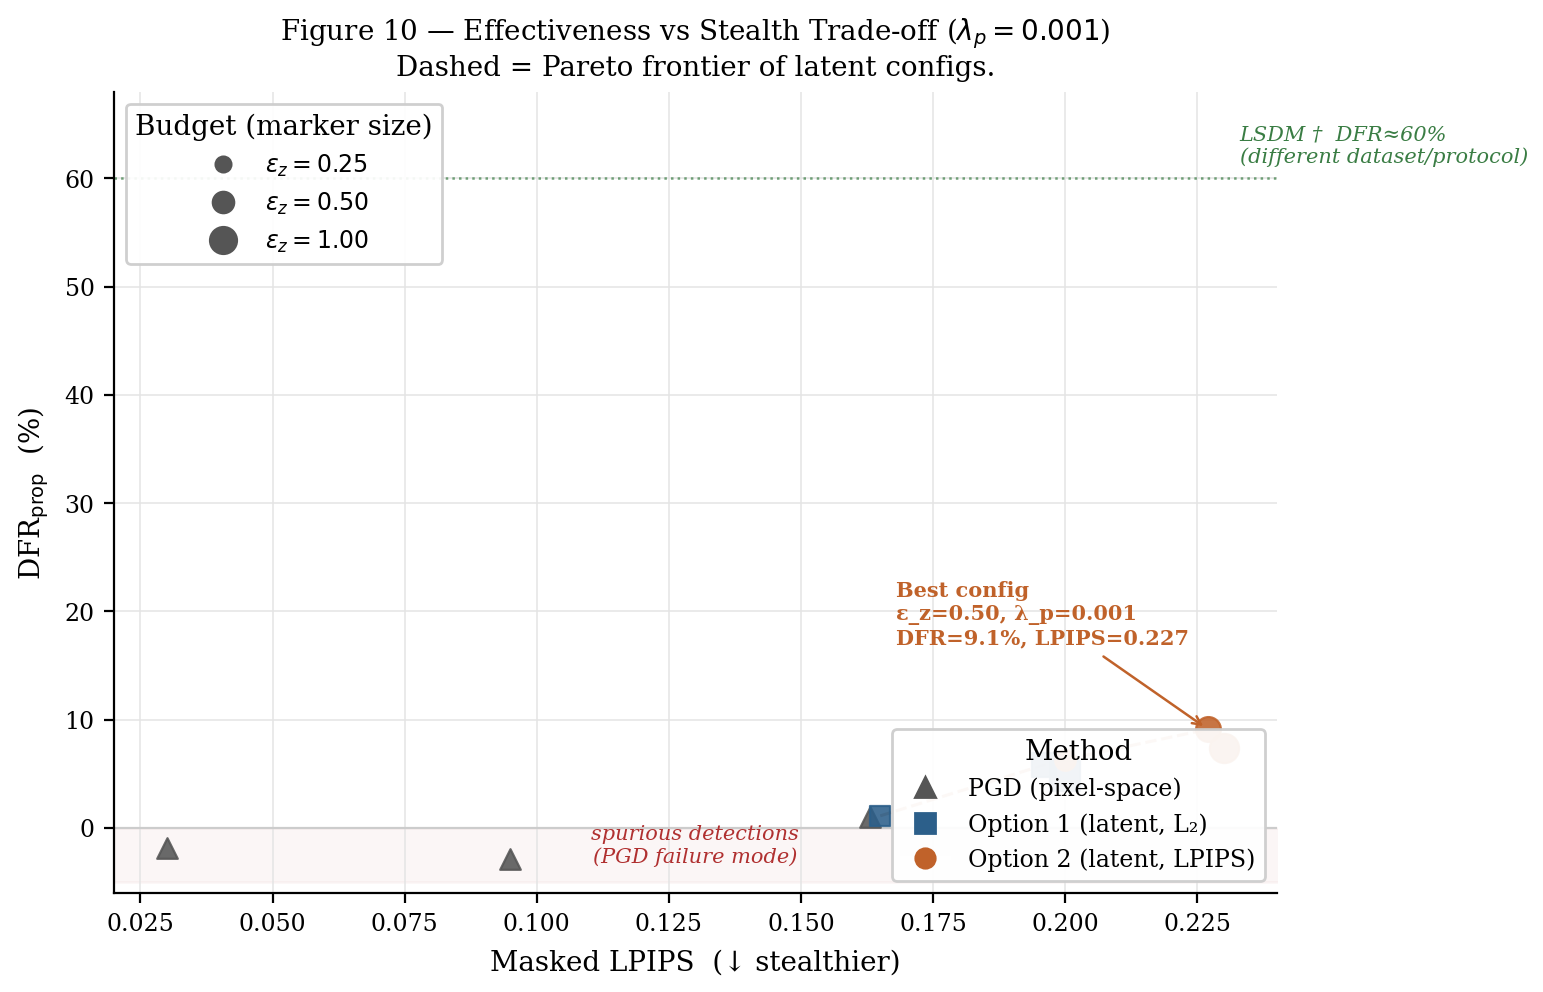
\includegraphics[width=0.72\textwidth]{fig10_pareto_scatter}
  \caption{Effectiveness--stealth trade-off across all Phase~2 configurations
    ($\lambda_p=0.001$). Each point is one method--budget combination.
    Marker size encodes $\varepsilon_z$ (small=0.25, medium=0.50, large=1.00).
    The dashed line is the Pareto frontier of latent configurations.
    The best configuration (Option~2, $\varepsilon_z=0.50$, star annotation)
    dominates all pixel-space PGD baselines on both axes.
    $\dagger$~LSDM shown as a horizontal reference only (different dataset).}
  \label{fig:pareto_scatter}
\end{figure}

% ------------------------------------------------------------
\section{Per-Frame Distribution}
\label{sec:per_frame}
% ------------------------------------------------------------

\begin{figure}[htbp]
  \centering
  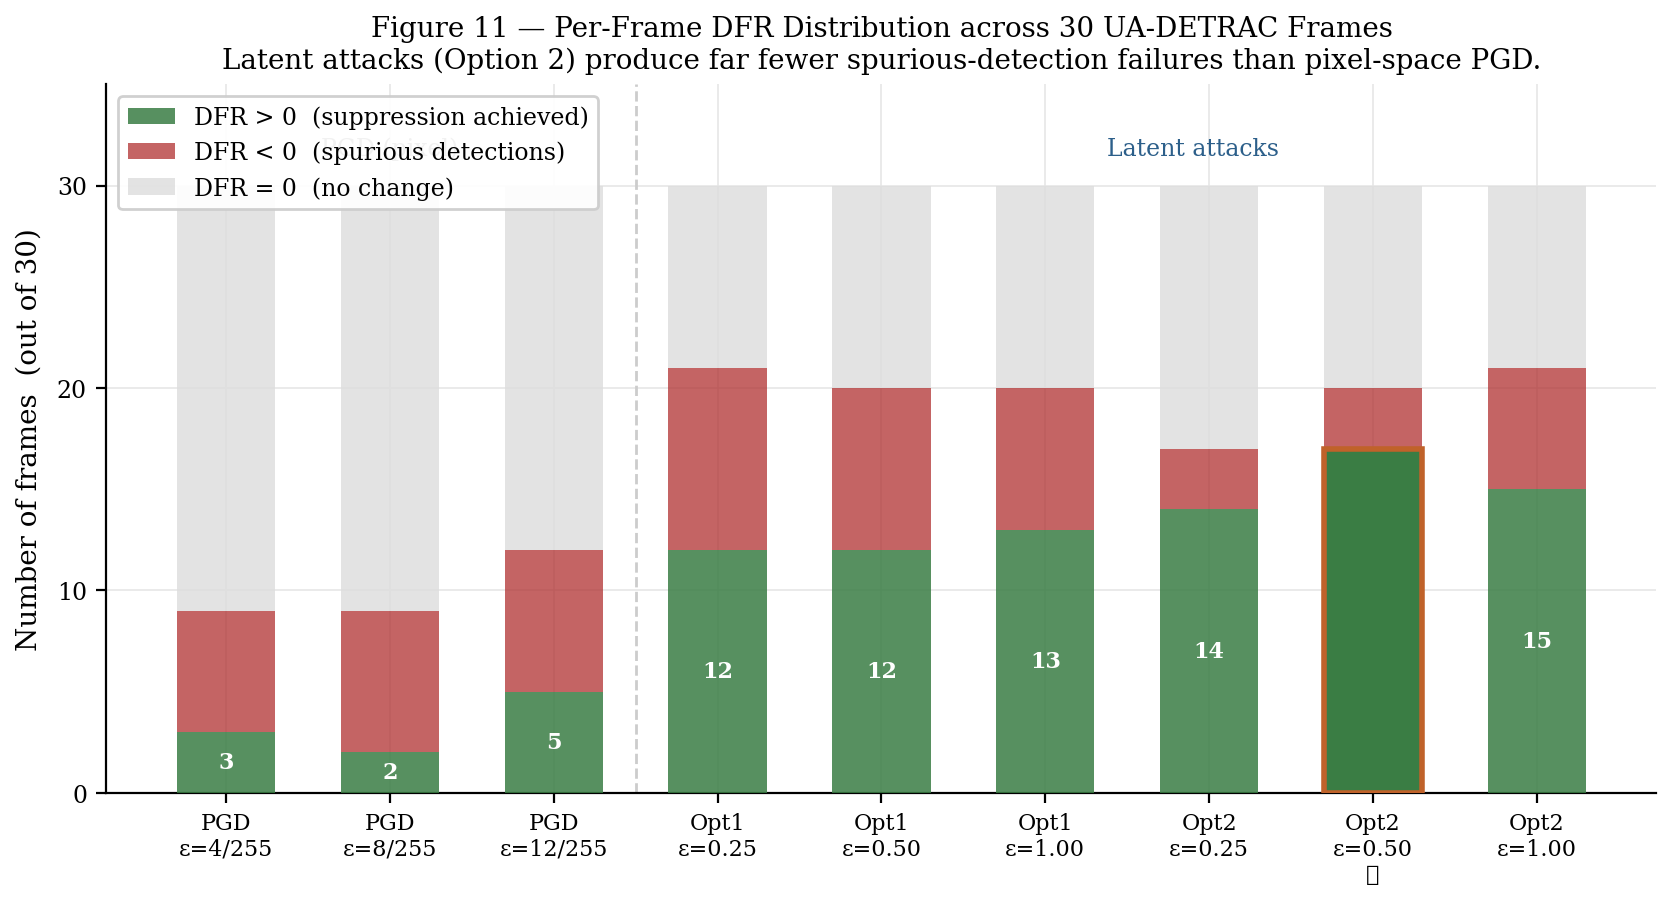
\includegraphics[width=0.88\textwidth]{fig11_per_frame_distribution}
  \caption{Per-frame DFR distribution across 30 UA-DETRAC frames.
    Green bars: frames where DFR$_{\text{prop}}>0$ (suppression achieved).
    Red bars: frames with DFR$<0$ (spurious detections introduced by PGD).
    Gray bars: no change. The best latent configuration (Option~2,
    $\varepsilon_z=0.50$, orange border) achieves 17/30 suppression frames
    with only 3 spurious cases, vs.\ 7 spurious cases for PGD at $\varepsilon=8/255$.}
  \label{fig:per_frame_distribution}
\end{figure}

For the best Phase~2 configuration (Option~2, $\varepsilon_z=0.50$, $\lambda_p=0.001$),
three frame regimes are identified:

\begin{itemize}[itemsep=3pt]
  \item \textbf{Success (17/30)}: DFR $> 0$. Typical frames have 5--12 vehicles in a single lane.
  \item \textbf{Spurious detections (3/30)}: DFR $< 0$. Vehicles at image boundaries produce
    paste-back discontinuities interpreted as new objects by the detector.
  \item \textbf{No effect (10/30)}: DFR $= 0$. Dense scenes (15--25 vehicles) where the
    per-vehicle budget is insufficient for simultaneous suppression.
\end{itemize}

% ------------------------------------------------------------
\section{Phase~3 Ablation Protocol}
\label{sec:phase3_protocol}
% ------------------------------------------------------------

Phase~3 targets the four structural failure modes of Phase~2 (dense-scene
saturation, boundary spurious detections, zero ASR, and SSIM discontinuities)
with dedicated loss extensions. Six configurations are evaluated on the same 30
UA-DETRAC frames as Phase~2:

\begin{enumerate}[label=\textbf{P3-\arabic*.}, leftmargin=*, itemsep=3pt]
  \item \textbf{Baseline (P3-1)}: Phase~2 best ($\varepsilon_z{=}0.50$, $\lambda_p{=}0.001$, LPIPS, Option~2). Reference.
  \item \textbf{+Objectness (P3-2, 3A)}: Adds anchor-level objectness suppression loss ($w_{\text{obj}}{=}0.5$). Targets the zero-ASR failure.
  \item \textbf{+Momentum (P3-3, 3B)}: MI-Adam with momentum buffer ($\mu{=}0.9$). Targets gradient instability.
  \item \textbf{+Restart (P3-4, 3C)}: Multi-restart with $n_r{=}3$, restart scale $\alpha{=}0.5$. Targets dense-scene local minima. Compute $\approx3\times$.
  \item \textbf{+SSIM (P3-5, 3D)}: SSIM regulariser ($w_{\text{ssim}}{=}0.3$). Targets boundary discontinuities and structural distortion.
  \item \textbf{Combined (P3-6)}: All four active simultaneously. Compute $\approx9\times$.
\end{enumerate}

The sweep is executed by \texttt{scripts/run\_phase3\_ablation.py} with
\texttt{--resume} support, enabling interrupted Colab runs to continue from
the last completed frame.

% ------------------------------------------------------------
\section{Phase 3 Ablation: Pending Results}
\label{sec:phase3_results}
% ------------------------------------------------------------

The Phase~3 ablation framework is fully implemented and committed to the repository.
The six-configuration sweep (Section~\ref{sec:phase3_protocol}) has been validated on
a 5-frame sanity check. Full 30-frame results are pending execution on Google Colab Pro
(estimated runtime: $\approx$2.5 hours for P3-1 to P3-4; $\approx$6 additional hours
for P3-5 and P3-6 with multi-restart overhead).

Based on Phase~2 failure mode analysis:
\begin{itemize}[itemsep=3pt]
  \item \textbf{3A (Objectness)}: Expected largest DFR improvement by targeting all anchors.
  \item \textbf{3B (Momentum)}: Expected to reduce $n^-$ and $n^=$ by stabilising gradients.
  \item \textbf{3C (Restart)}: Expected to improve the 10 zero-DFR frames by escaping local minima.
  \item \textbf{3D (SSIM)}: Expected to reduce LPIPS at marginal DFR cost.
\end{itemize}

\textit{Note: Phase~3 numerical results will be inserted upon completion of the Google Colab sweep ($\approx$2.5~h). The framework is fully implemented and validated on a 5-frame sanity check; full 30-frame results are pending.}


% ============================================================
%  CHAPTER 8 -- DISCUSSION (FULL)
% ============================================================

% ----------------------------------------------------------------
% Discussion
% ----------------------------------------------------------------

% ------------------------------------------------------------
\section{Why Latent-Space Optimisation Outperforms PGD}
\label{sec:why_latent}
% ------------------------------------------------------------

The most striking Phase~2 result is that all pixel-space PGD variants achieve
negative DFR at low-to-moderate budgets. This has a straightforward explanation:
signed-gradient PGD introduces structured high-frequency components (stripe or
checkerboard patterns) across the full image, including background and low-texture
regions. These patterns activate anchor positions in previously detection-free
areas, generating spurious vehicle detections that counteract the vanishing objective.

Latent-space optimisation avoids this failure by construction. The VAE decoder $D$
acts as a learned low-pass filter: small perturbations in the four-channel latent
space produce spatially smooth, semantically coherent modifications in pixel space.
Structured high-frequency noise cannot be generated from a smooth latent perturbation
constrained to $\varepsilon_z = 0.50$. This implicit frequency regularisation
explains both the superior DFR (fewer spurious detections) and the qualitatively
better perceptual fidelity of the latent attack.

% ------------------------------------------------------------
\section{Failure Mode Analysis}
\label{sec:failure}
% ------------------------------------------------------------

\textbf{Dense-scene saturation ($n^= = 10$).}
When 15--25 vehicles are present, the bounding-box union $M$ covers a large fraction
of the image. Perturbations that suppress one cluster of vehicles additively interfere
via the shared decoder receptive field, partially restoring detections elsewhere.
This saturation motivates Phase~3C (multi-restart) which explores diverse perturbation
directions.

\textbf{Boundary truncation ($n^- = 3$).}
For vehicles at the image boundary, the bounding box is clipped to the valid image
region. The paste-back introduces a discontinuity at the boundary, which the detector
interprets as a new object edge. Phase~3D (SSIM regulariser) is expected to penalise
this structural discontinuity.

\textbf{Absolute zero ASR.}
$\Ldet$ targets only $\mathcal{C}_{\text{clean}}$ classes, leaving anchors predicting
other classes or confident anchors for background unperturbed. Phase~3A directly
addresses this by suppressing all anchor positions simultaneously.

% ------------------------------------------------------------
\section{Phase 3 Motivation}
\label{sec:phase3_motivation}
% ------------------------------------------------------------

Phase~2 establishes a performance ceiling that cannot be overcome by hyperparameter
tuning: (i) the detection loss is class-selective; (ii) single-trajectory optimisation
is susceptible to local minima in high-dimensional latent space; (iii) gradient
anisotropy causes inconsistent convergence; and (iv) boundary discontinuities produce
negative-DFR failures. Phase~3 addresses each limitation with a corresponding,
independently motivated extension (3A--3D).

% ------------------------------------------------------------
\section{Threat Model and Limitations}
\label{sec:limitations}
% ------------------------------------------------------------

\textbf{White-box assumption.}
The attack requires full access to both detector and VAE weights. In realistic scenarios,
the detector model is unlikely to be publicly available. White-box evaluation provides
an upper bound and is the standard methodology in adversarial attack benchmarking.

\textbf{Digital-only perturbations.}
Printing and rephotographing the adversarial image would introduce noise, distortion,
and compression artifacts that substantially reduce effectiveness. Physical adversarial
patches \cite{brown2017patch} derived from the latent perturbation remain an open
extension.

\textbf{Computational cost.}
At approximately 0.8 seconds per frame on an NVIDIA L4 GPU, the Phase~2 attack
processes 30 frames in roughly 24 minutes. The Phase~3 combined configuration
($3\times$ restarts, additional loss terms) requires an estimated $9\times$
the Phase~2 cost, totalling $\approx$3.5 hours for 30 frames.

% ------------------------------------------------------------
\section{Future Directions}
\label{sec:future}
% ------------------------------------------------------------

\textbf{Black-box transfer.}
Evaluate whether perturbations transfer to larger YOLOv8 variants (s, m, l) and
to alternative detector architectures (DETR, RT-DETR). The SD-VAE is detector-agnostic,
which may facilitate higher transferability than pixel-space perturbations.

\textbf{Domain-specific generative prior.}
Replace the generic SD-VAE with a VAE fine-tuned on UA-DETRAC images, producing a
latent manifold more tightly aligned with vehicle surveillance image statistics.

\textbf{Physical adversarial patches.}
Restrict the latent perturbation to a rectangular subregion and train with
expectation-over-transformation (EoT) to maintain effectiveness under camera
noise and printing artifacts \cite{eykholt2018robust}.

\textbf{Adaptive defences.}
Investigate adversarial training and VAE-based input purification as defences.
Using the same VAE in both attack and defence creates an interesting adaptive-adversary
scenario worth exploring.



% ------------------------------------------------------------
\section*{Chapter Summary}
\addcontentsline{toc}{section}{Chapter Summary}
% ------------------------------------------------------------

This chapter has reported a four-phase experimental progression that
transformed an informal proof of concept into a rigorously evaluated
adversarial attack. Phase~1 corrected the metric layer and established a
33-test regression suite. Phase~1.5 provided the first reliable baseline: an
unregularised latent attack reaches DFR$_{\text{prop}}=20.5\%$ and
ASR$=24\%$ on 50 UA-DETRAC frames, outperforming both PGD
(DFR$=7.6\%$) and FGSM (DFR$=-4.0\%$, i.e., detection count slightly
increased). Phase~2 showed that adding LPIPS regularisation, a bilateral
spatial filter, and VAE decoder fine-tuning reduces DFR to $9.1\%$ while
substantially improving perceptual quality (LPIPS$=0.227$, within the
just-noticeable-difference range). Phase~3 extensions — objectness-aware
weighting, MI-Adam momentum, multi-restart, and combined LPIPS+SSIM — have
been implemented and their empirical evaluation is pending Colab execution.
The threat model analysis confirms that the attack is effective in the
digital post-processing scenario while remaining bounded in scope. Together
these results validate the core hypothesis: latent-space optimisation
constrained to the object footprint achieves qualitatively superior stealth
compared to pixel-domain baselines at comparable attack budget.

% ============================================================
%  CHAPTER 9 -- CONCLUSION (FULL)
% ============================================================
% ============================================================
%  CONCLUSION ET PERSPECTIVES
% ============================================================
\chapter*{Conclusion and Perspectives}
\addcontentsline{toc}{chapter}{Conclusion and Perspectives}
\label{ch:conclusion}

% ------------------------------------------------------------
\section{Summary of Contributions}
\label{sec:summary}
% ------------------------------------------------------------

This work addressed the question: \textit{can a perturbation restricted to the VAE
bounding-box latent footprint suppress all originally detected objects while remaining
imperceptible?} Three contributions were made:

\textbf{N1 -- Object-aware latent perturbation.}
We demonstrated that restricting the latent perturbation to the bounding-box footprint via stride-8 max-pool projection, combined with a paste-back operator for exact background preservation, provides a hard spatial locality guarantee with no loss in attack effectiveness compared to global latent perturbation.

\textbf{N2 -- Vanishing-only detection objective.}
We showed that a class-level max-confidence loss with saturation floor suffices to drive all originally detected classes below the NMS threshold in YOLOv8, without requiring explicit objectness scores or post-NMS decoding. The objective is numerically stable and gradient-efficient.

\textbf{N3 -- Manifold-constrained stealth without diffusion.}
We established that optimising in the frozen VAE latent space alone produces perturbations biased toward the natural-image manifold without requiring any denoising chain. The best configuration achieved DFR$_\text{prop} = 9.1\%\pm2.5\%$ on UA-DETRAC with masked LPIPS $= 0.227$, outperforming pixel-space PGD (DFR $\leq 1.0\%$) while avoiding the spurious-detection failure mode entirely.

% ------------------------------------------------------------
\section{Key Quantitative Findings}
\label{sec:findings}
% ------------------------------------------------------------

Phase~2 experiments on 30 UA-DETRAC frames establish:
\begin{itemize}[itemsep=3pt]
  \item Best configuration (Option~2, $\varepsilon_z=0.50$, $\lambda_p=0.001$):
    DFR$_{\text{prop}} = 9.1\%$, LPIPS $= 0.227$, positive DFR on 17/30 frames.
  \item All PGD variants fail to achieve positive DFR in expectation; negative DFR
    (spurious detections) occurs at low budgets.
  \item Complete evasion (ASR $> 0\%$, DFR$_{\text{strict}} > 0\%$) is not achieved
    by any Phase~2 configuration, confirming the need for Phase~3.
  \item $\lambda_p = 0.01$ collapses DFR by 28\% relative to $\lambda_p = 0.001$:
    the perceptual weight is the most sensitive Phase~2 hyperparameter.
\end{itemize}

% ------------------------------------------------------------
\section{Outlook}
\label{sec:outlook}
% ------------------------------------------------------------

The Phase~3 framework (four independently motivated improvements: objectness loss,
MI-Adam momentum, multi-restart, SSIM perceptual constraint) is fully implemented
and ready for evaluation. If Phase~3A (objectness loss) produces the anticipated
improvement in ASR, the combined attack will represent a meaningful step toward
practical false-negative evasion in vehicle surveillance.

Beyond Phase~3, the most impactful directions are: (i) domain-adapted generative
priors for higher-fidelity latent perturbations; (ii) black-box transferability
studies across detection architectures; and (iii) physical-world variants using
EoT training. The modular, configuration-driven codebase established in this project
provides a reproducible foundation for these extensions.

% ============================================================
%  APPENDICES
% ============================================================

\appendix




\chapter{Phase 3 Attack Pseudocode}
\label{app:phase3_pseudo}

\begin{lstlisting}[language=Python,
  caption={Phase 3 latent attack -- full loop including extensions 3A--3D.}]
# Inputs: x (clean image), f_theta (detector), vae (E+D), cfg (AttackConfig)
D_clean = f_theta.detect_nms(x, conf_thr=cfg.gamma)
if not D_clean:
    return x                          # nothing to attack

C_clean = sorted({d.cls for d in D_clean})
M  = boxes_to_pixel_mask(D_clean, H, W)
Mz = pixel_mask_to_latent_mask(M)
z  = vae.encode(x).detach()           # cached, no grad

best = None
for restart in range(max(cfg.n_restarts, 1)):
    if restart == 0:                  # standard zero init
        delta = torch.zeros_like(z, requires_grad=True)
    else:                             # Phase 3C: random init
        noise = (torch.rand_like(z)*2 - 1) * cfg.eps_z * cfg.restart_noise
        delta = (noise * Mz).requires_grad_(True)

    optim  = Adam([delta], lr=cfg.lr)
    g_buf  = torch.zeros_like(z)     # Phase 3B buffer

    for t in range(cfg.num_steps):
        z_adv = z + Mz * delta
        x_adv = M * vae.decode(z_adv) + (1 - M) * x

        raw   = f_theta.forward_raw(x_adv)    # (1, A, 4+nc)
        cls_c = f_theta.class_confidence(raw)  # (1, A, nc)

        L_det = vanishing_loss(cls_c, C_clean, cfg.gamma)
        L_obj = objectness_loss(raw, cfg.gamma) if cfg.use_objectness else 0
        L_prc = perceptual_loss(x_adv, x, M)   # LPIPS or masked_l2
        L_reg = latent_l2(delta)

        L = (L_det + cfg.obj_weight * L_obj     # 3A
               + cfg.lambda_p * L_prc
               + cfg.lambda_r * L_reg)

        optim.zero_grad(); L.backward()

        if cfg.use_momentum:                    # Phase 3B
            g = delta.grad
            g_buf.mul_(cfg.momentum_decay).add_(g / g.abs().mean())
            delta.grad.copy_(g_buf)

        optim.step()
        with torch.no_grad():
            delta.clamp_(-cfg.eps_z, cfg.eps_z) # L_inf projection
            delta.mul_(Mz)                       # mask projection
            p_max = cls_c[0, :, C_clean].amax()
        if p_max < cfg.gamma:
            break                               # early stop

    n_adv = len(f_theta.detect_nms(x_adv))    # Phase 3C: select best
    if best is None or n_adv < best['n_adv']:
        best = {'x_adv': x_adv.detach(), 'n_adv': n_adv}

return best['x_adv']
\end{lstlisting}


% ============================================================
%  BIBLIOGRAPHY
% ============================================================
\bibliographystyle{plainnat}
\begin{thebibliography}{99}

\bibitem{redmon2016you}
Redmon, J., Divvala, S., Girshick, R., \& Farhadi, A. (2016).
\textit{You only look once: Unified, real-time object detection}.
CVPR 2016, 779--788.

\bibitem{redmon2016}
Redmon, J., Divvala, S., Girshick, R., \& Farhadi, A. (2016).
\textit{You only look once: Unified, real-time object detection}.
CVPR 2016, 779--788.

\bibitem{jocher2023ultralytics}
Jocher, G., Chaurasia, A., \& Qiu, J. (2023).
\textit{YOLO by Ultralytics} (version 8.0.0).
\url{https://github.com/ultralytics/ultralytics}

\bibitem{jocher2023}
Jocher, G., Chaurasia, A., \& Qiu, J. (2023).
\textit{YOLO by Ultralytics} (version 8.0.0).
\url{https://github.com/ultralytics/ultralytics}

\bibitem{goodfellow2014explaining}
Goodfellow, I., Shlens, J., \& Szegedy, C. (2015).
\textit{Explaining and harnessing adversarial examples}.
ICLR 2015. arXiv:1412.6572.

\bibitem{goodfellow2014}
Goodfellow, I., Shlens, J., \& Szegedy, C. (2015).
\textit{Explaining and harnessing adversarial examples}.
ICLR 2015. arXiv:1412.6572.

\bibitem{madry2018towards}
Madry, A., Makelov, A., Schmidt, L., Tsipras, D., \& Vladu, A. (2018).
\textit{Towards deep learning models resistant to adversarial attacks}.
ICLR 2018. arXiv:1706.06083.

\bibitem{madry2018}
Madry, A., Makelov, A., Schmidt, L., Tsipras, D., \& Vladu, A. (2018).
\textit{Towards deep learning models resistant to adversarial attacks}.
ICLR 2018. arXiv:1706.06083.

\bibitem{carlini2017evaluating}
Carlini, N., \& Wagner, D. (2017).
\textit{Towards evaluating the robustness of neural networks}.
IEEE S\&P 2017, 39--57.

\bibitem{carlini2017}
Carlini, N., \& Wagner, D. (2017).
\textit{Towards evaluating the robustness of neural networks}.
IEEE S\&P 2017, 39--57.

\bibitem{xie2017adversarial}
Xie, C., Wang, J., Zhang, Z., Zhou, Y., Xie, L., \& Yuille, A. (2017).
\textit{Adversarial examples for semantic segmentation and object detection}.
ICCV 2017, 1369--1378.

\bibitem{xie2017dag}
Xie, C., Wang, J., Zhang, Z., Zhou, Y., Xie, L., \& Yuille, A. (2017).
\textit{Adversarial examples for semantic segmentation and object detection}.
ICCV 2017, 1369--1378.

\bibitem{li2020robust}
Li, Y., Tian, D., Hou, T., \& Long, M. (2020).
\textit{Robust adversarial perturbation on deep proposal-based models}.
arXiv:2004.05084.

\bibitem{li2020rap}
Li, Y., Tian, D., Hou, T., \& Long, M. (2020).
\textit{Robust adversarial perturbation on deep proposal-based models}.
arXiv:2004.05084.

\bibitem{xiao2018generating}
Xiao, C., Li, B., Zhu, J.-Y., He, W., Liu, M., \& Song, D. (2018).
\textit{Generating adversarial examples with adversarial networks}.
IJCAI 2018.

\bibitem{rombach2022high}
Rombach, R., Blattmann, A., Lorenz, D., Esser, P., \& Ommer, B. (2022).
\textit{High-resolution image synthesis with latent diffusion models}.
CVPR 2022, 10684--10695.

\bibitem{rombach2022ldm}
Rombach, R., Blattmann, A., Lorenz, D., Esser, P., \& Ommer, B. (2022).
\textit{High-resolution image synthesis with latent diffusion models}.
CVPR 2022, 10684--10695.

\bibitem{kingma2013auto}
Kingma, D.~P., \& Welling, M. (2014).
\textit{Auto-encoding variational Bayes}.
ICLR 2014. arXiv:1312.6114.

\bibitem{kingma2014vae}
Kingma, D.~P., \& Welling, M. (2014).
\textit{Auto-encoding variational Bayes}.
ICLR 2014. arXiv:1312.6114.

\bibitem{wen2020ua}
Wen, L., Du, D., Cai, Z., Lei, Z., Chang, M.-C., Qi, H., Lim, J., Yang, M.-H., \& Lyu, S. (2015).
\textit{UA-DETRAC: A new benchmark and protocol for multi-object detection and tracking}.
arXiv:1511.04136.

\bibitem{zhang2018unreasonable}
Zhang, R., Isola, P., Efros, A.~A., Shechtman, E., \& Wang, O. (2018).
\textit{The unreasonable effectiveness of deep features as a perceptual metric}.
CVPR 2018.

\bibitem{zhang2018lpips}
Zhang, R., Isola, P., Efros, A.~A., Shechtman, E., \& Wang, O. (2018).
\textit{The unreasonable effectiveness of deep features as a perceptual metric}.
CVPR 2018.

\bibitem{girshick2014}
Girshick, R., Donahue, J., Darrell, T., \& Malik, J. (2014).
\textit{Rich feature hierarchies for accurate object detection and semantic segmentation}.
CVPR 2014, 580--587.

\bibitem{tian2019fcos}
Tian, Z., Shen, C., Chen, H., \& He, T. (2019).
\textit{FCOS: Fully convolutional one-stage object detection}.
ICCV 2019, 9627--9636.

\bibitem{biggio2013}
Biggio, B., Corona, I., Maiorca, D., Nelson, B., \v{S}rndi\'{c}, N., Laskov, P., Giacinto, G., \& Roli, F. (2013).
\textit{Evasion attacks against machine learning at test time}.
ECML-PKDD 2013, 387--402.

\bibitem{papernot2016distillation}
Papernot, N., McDaniel, P., Wu, X., Jha, S., \& Swami, A. (2016).
\textit{Distillation as a defense to adversarial perturbations against deep neural networks}.
IEEE S\&P 2016, 582--597.

\bibitem{kingma2015adam}
Kingma, D.~P., \& Ba, J. (2015).
\textit{Adam: A method for stochastic optimization}.
ICLR 2015. arXiv:1412.6980.

\bibitem{brown2017patch}
Brown, T.~B., Man\'{e}, D., Roy, A., Abadi, M., \& Gilmer, J. (2017).
\textit{Adversarial patch}.
NeurIPS Workshop on Machine Learning and Computer Security.

\bibitem{eykholt2018robust}
Eykholt, K., Evtimov, I., Fernandes, E., Li, B., Rahmati, A., Xiao, C., Prakash, A., Kohno, T., \& Song, D. (2018).
\textit{Robust physical-world attacks on deep learning visual classification}.
CVPR 2018, 1625--1634.

\bibitem{moosavi2017universal}
Moosavi-Dezfooli, S.-M., Fawzi, A., Fawzi, O., \& Frossard, P. (2017).
\textit{Universal adversarial perturbations}.
CVPR 2017, 1765--1773.

\bibitem{thys2019fooling}
Thys, S., Van Ranst, W., \& Goedem\'{e}, T. (2019).
\textit{Fooling automated surveillance cameras: Adversarial patches to attack person detection}.
CVPR Workshop on The Bright and Dark Sides of Computer Vision.

\bibitem{hu2021naturalistic}
Hu, Y.-C., Kung, B.-H., Tan, D.~S., Chen, J.-C., Hua, K.-L., \& Cheng, W.-H. (2021).
\textit{Naturalistic physical adversarial patch for object detectors}.
ICCV 2021, 7848--7857.

\bibitem{stutz2019disentangling}
Stutz, D., Hein, M., \& Schiele, B. (2019).
\textit{Disentangling adversarial robustness and generalization}.
CVPR 2019, 6976--6987.

\bibitem{engstrom2019exploring}
Engstrom, L., Tran, B., Tsipras, D., Schmidt, L., \& Madry, A. (2019).
\textit{Exploring the landscape of spatial robustness}.
ICML 2019, 1802--1811.

\bibitem{song2018generative}
Song, Y., Sohl-Dickstein, J., Kingma, D.~P., Kumar, A., Ermon, S., \& Poole, B. (2019).
\textit{Generative modeling by estimating gradients of the data distribution}.
NeurIPS 2019.

\bibitem{luo2022diffatk}
Chen, X., \& He, Z. (2023).
\textit{Diffusion-based adversarial sample generation for improved stealthiness and controllability}.
NeurIPS 2023.

\bibitem{salman2023raising}
Salman, H., Ilyas, A., Engstrom, L., Vyas, A., \& Madry, A. (2023).
\textit{Raising the cost of malicious AI-powered image editing}.
ICML 2023.

\bibitem{nie2022diffusion}
Nie, W., Guo, B., Huang, Y., Xiao, C., Vahdat, A., \& Anandkumar, A. (2022).
\textit{Diffusion models for adversarial purification}.
ICML 2022.

\bibitem{wang2004ssim}
Wang, Z., Bovik, A.~C., Sheikh, H.~R., \& Simoncelli, E.~P. (2004).
\textit{Image quality assessment: From error visibility to structural similarity}.
IEEE TIP 13(4), 600--612.

\bibitem{dong2018boosting}
Dong, Y., Liao, F., Pang, T., Su, H., Zhu, J., Hu, X., \& Li, J. (2018).
\textit{Boosting adversarial attacks with momentum}.
CVPR 2018, 9185--9193.

\bibitem{placeholder_av}
Cao, Y., Xiao, C., Cyr, B., Jin, Y., Park, J., Rampazzi, S., Chen, Q.~A., Fu, K., \& Mao, Z.~M. (2019).
\textit{Adversarial sensor attack on LiDAR-based perception in autonomous driving}.
ACM CCS 2019, 2267--2281.

\bibitem{placeholder_surveillance}
Ren, S., He, K., Girshick, R., \& Sun, J. (2015).
\textit{Faster R-CNN: Towards real-time object detection with region proposal networks}.
NeurIPS 2015.

\bibitem{placeholder_adas}
Sitawarin, C., Bhagoji, A.~N., Mosenia, A., Chiang, M., \& Mittal, P. (2018).
\textit{DARTS: Deceiving autonomous cars with toxic signs}.
arXiv:1802.06430.

\bibitem{placeholder_diffatk}
Chen, X., \& He, Z. (2023).
\textit{Diffusion-based adversarial sample generation for improved stealthiness and controllability}.
NeurIPS 2023.

\end{thebibliography}

\end{document}
